%%
%% This is file `sample-acmlarge.tex',
%% generated with the docstrip utility.
%%
%% The original source files were:
%%
%% samples.dtx  (with options: `all,journal,bibtex,acmlarge')
%% 
%% IMPORTANT NOTICE:
%% 
%% For the copyright see the source file.
%% 
%% Any modified versions of this file must be renamed
%% with new filenames distinct from sample-acmlarge.tex.
%% 
%% For distribution of the original source see the terms
%% for copying and modification in the file samples.dtx.
%% 
%% This generated file may be distributed as long as the
%% original source files, as listed above, are part of the
%% same distribution. (The sources need not necessarily be
%% in the same archive or directory.)
%%
%%
%% Commands for TeXCount
%TC:macro \cite [option:text,text]
%TC:macro \citep [option:text,text]
%TC:macro \citet [option:text,text]
%TC:envir table 0 1
%TC:envir table* 0 1
%TC:envir tabular [ignore] word
%TC:envir displaymath 0 word
%TC:envir math 0 word
%TC:envir comment 0 0
%%
%%
%% The first command in your LaTeX source must be the \documentclass
%% command.
%%
%% For submission and review of your manuscript please change the
%% command to \documentclass[manuscript, screen, review]{acmart}.
%%
%% When submitting camera ready or to TAPS, please change the command
%% to \documentclass[sigconf]{acmart} or whichever template is required
%% for your publication.
%%
%%
\documentclass[acmlarge]{acmart}

%%
%% \BibTeX command to typeset BibTeX logo in the docs
\AtBeginDocument{%
  \providecommand\BibTeX{{%
    Bib\TeX}}}

%% Rights management information.  This information is sent to you
%% when you complete the rights form.  These commands have SAMPLE
%% values in them; it is your responsibility as an author to replace
%% the commands and values with those provided to you when you
%% complete the rights form.
\setcopyright{acmlicensed}
\copyrightyear{2018}
\acmYear{2018}
\acmDOI{XXXXXXX.XXXXXXX}


%%
%% These commands are for a JOURNAL article.
\acmJournal{POMACS}
\acmVolume{37}
\acmNumber{4}
\acmArticle{111}
\acmMonth{8}

%%
%% Submission ID.
%% Use this when submitting an article to a sponsored event. You'll
%% receive a unique submission ID from the organizers
%% of the event, and this ID should be used as the parameter to this command.
%%\acmSubmissionID{123-A56-BU3}

%%
%% For managing citations, it is recommended to use bibliography
%% files in BibTeX format.
%%
%% You can then either use BibTeX with the ACM-Reference-Format style,
%% or BibLaTeX with the acmnumeric or acmauthoryear sytles, that include
%% support for advanced citation of software artefact from the
%% biblatex-software package, also separately available on CTAN.
%%
%% Look at the sample-*-biblatex.tex files for templates showcasing
%% the biblatex styles.
%%

%%
%% The majority of ACM publications use numbered citations and
%% references.  The command \citestyle{authoryear} switches to the
%% "author year" style.
%%
%% If you are preparing content for an event
%% sponsored by ACM SIGGRAPH, you must use the "author year" style of
%% citations and references.
%% Uncommenting
%% the next command will enable that style.
%%\citestyle{acmauthoryear}


%%
%% end of the preamble, start of the body of the document source.
\begin{document}

%%
%% The "title" command has an optional parameter,
%% allowing the author to define a "short title" to be used in page headers.
\title{Extractive Text Summarization Using Word Similarity-based Spectral Clustering}

%%
%% The "author" command and its associated commands are used to define
%% the authors and their affiliations.
%% Of note is the shared affiliation of the first two authors, and the
%% "authornote" and "authornotemark" commands
%% used to denote shared contribution to the research.
\author{Fahim Morshed}
%\authornote{Both authors contributed equally to this research.}
\email{f.morshed.opee@gmail.com}
%\orcid{1234-5678-9012}
\affiliation{%
	\institution{Institute of Information Technology, University of Dhaka}
	\city{Dhaka}
	%\state{Ohio}
	\country{Bangladesh}
}

\author{Md. Abdur Rahman}
\affiliation{%
	\institution{Centre for Advanced Research in Science, University of Dhaka}
	\city{Dhaka}
	\country{Bangladesh}}
\email{mukul.arahman@gmail.com}

\author{Sumon Ahmed}
%\authornotemark[1]
\email{sumon@du.ac.bd}
\affiliation{%
  \institution{Institute of Information Technology, University of Dhaka}
  \city{Dhaka}
  %\state{Ohio}
  \country{Bangladesh}
}



\begin{comment}
	\author{Valerie B\'eranger}
	\affiliation{%
		\institution{Inria Paris-Rocquencourt}
		\city{Rocquencourt}
		\country{France}
	}
	
	\author{Aparna Patel}
	\affiliation{%
		\institution{Rajiv Gandhi University}
		\city{Doimukh}
		\state{Arunachal Pradesh}
		\country{India}}
	
	\author{Huifen Chan}
	\affiliation{%
		\institution{Tsinghua University}
		\city{Haidian Qu}
		\state{Beijing Shi}
		\country{China}}
	
	\author{Charles Palmer}
	\affiliation{%
		\institution{Palmer Research Laboratories}
		\city{San Antonio}
		\state{Texas}
		\country{USA}}
	\email{cpalmer@prl.com}
	
	\author{John Smith}
	\affiliation{%
		\institution{The Th{\o}rv{\"a}ld Group}
		\city{Hekla}
		\country{Iceland}}
	\email{jsmith@affiliation.org}
	
	\author{Julius P. Kumquat}
	\affiliation{%
		\institution{The Kumquat Consortium}
		\city{New York}
		\country{USA}}
	\email{jpkumquat@consortium.net}
\end{comment}


%%
%% By default, the full list of authors will be used in the page
%% headers. Often, this list is too long, and will overlap
%% other information printed in the page headers. This command allows
%% the author to define a more concise list
%% of authors' names for this purpose.
\renewcommand{\shortauthors}{Morshed et al.}

%%
%% The abstract is a short summary of the work to be presented in the
%% article.
\begin{abstract}
  Extractive Text Summarization is the process of picking the best parts of a  larger text without losing any key information. This is really necessary in this day and age to get concise information faster due to digital information overflow. Previous attempts at extractive text summarization, specially in Bengali, either relied on TF-IDF or used naive similarity measures both of these suffers expressing semantic relationship correctly. The objective of this paper is to develop an extractive text summarization method  for Bengali language, that uses the latest NLP techniques and extended to other low resource languages. We developed a word Similarity-based Spectral Clustering (WSbSC) method for  Bengali extractive text summarization. It extracts key sentences by grouping semantically similar sentences into clusters  with a novel sentence similarity calculating algorithm. We took the geometric means of individual Gaussian similarity values using word embedding vectors to get the similarity between two sentences. Then, used TF-IDF ranking to pick the best sentence from each cluster. This method is tested on four datasets, and it outperformed other recent models by 43.2\% on average ROUGE scores (ranging from 2.5\% to 95.4\%). The method is also experimented on Turkish, Marathi and Hindi language and found that the performance on those languages often exceeded the performance of Bengali. In addition, a new high quality dataset is provided for text summarization evaluation. We, believe this research is a crucial addition to Bengali Natural Language Processing, that can easily be extended into other languages.
\end{abstract}

%%
%% The code below is generated by the tool at http://dl.acm.org/ccs.cfm.
%% Please copy and paste the code instead of the example below.
%%
\begin{CCSXML}
<ccs2012>
 <concept>
  <concept_id>00000000.0000000.0000000</concept_id>
  <concept_desc>Do Not Use This Code, Generate the Correct Terms for Your Paper</concept_desc>
  <concept_significance>500</concept_significance>
 </concept>
 <concept>
  <concept_id>00000000.00000000.00000000</concept_id>
  <concept_desc>Do Not Use This Code, Generate the Correct Terms for Your Paper</concept_desc>
  <concept_significance>300</concept_significance>
 </concept>
 <concept>
  <concept_id>00000000.00000000.00000000</concept_id>
  <concept_desc>Do Not Use This Code, Generate the Correct Terms for Your Paper</concept_desc>
  <concept_significance>100</concept_significance>
 </concept>
 <concept>
  <concept_id>00000000.00000000.00000000</concept_id>
  <concept_desc>Do Not Use This Code, Generate the Correct Terms for Your Paper</concept_desc>
  <concept_significance>100</concept_significance>
 </concept>
</ccs2012>
\end{CCSXML}

\ccsdesc[500]{Do Not Use This Code~Generate the Correct Terms for Your Paper}
\ccsdesc[300]{Do Not Use This Code~Generate the Correct Terms for Your Paper}
\ccsdesc{Do Not Use This Code~Generate the Correct Terms for Your Paper}
\ccsdesc[100]{Do Not Use This Code~Generate the Correct Terms for Your Paper}

%%
%% Keywords. The author(s) should pick words that accurately describe
%% the work being presented. Separate the keywords with commas.
\keywords{Do, Not, Us, This, Code, Put, the, Correct, Terms, for,
  Your, Paper}

\received{20 February 2007}
\received[revised]{12 March 2009}
\received[accepted]{5 June 2009}

%%
%% This command processes the author and affiliation and title
%% information and builds the first part of the formatted document.
\maketitle

\section{Introduction}\label{sec:introduction}
Text Summarization is the process of shortening a larger text without losing any key information to increase the readability and save time for the reader. But manually summarizing very large texts is a counter-productive task due to it being more time consuming and tedious. So, developing an Automatic Text Summarization (ATS) method that can summarize larger texts reliably is really necessary to alleviate this manual labour \cite{Widyassari-2022-rev-ats-tech-met}. 
%ATS is a major area of rapidly progressing Natural Language Processing (NLP) research due to the importance of summarization increasing significantly. This increase can be attributed to the information overflow in the digital era due to the trend of exponential growth of textual data in last few years \cite{2015-Forbes-80-created-last-2-years}. 
Using ATS to summarize textual data is thus becoming very important in various fields such as news articles, legal documents, health reports, research papers, social media contents etc. ATS helps the reader to quickly and efficiently get the essential information without needing to read through large amounts of texts \cite{wafaa-2021-summary-comprehensive-review}. So, ATS is being utilized in various fields, from automatic news summarization, content filtering, and recommendation systems to assisting legal professionals in going through long documents. And researchers in reviewing academic papers by condensing vast amount of informations. It can also play a critical role in personal assistants and chatbots, providing condensed information to users quickly and efficiently \cite{tas-2017-rev-text-sum-2}.\\

There are two main types of ATS: extractive and abstractive \cite{tas-2017-rev-text-sum-2}. Extractive summarization, which is the focus of this paper, works by selecting a subset from the source document, maintaining the original wording and sentence structure \cite{moratanch-2017-extractive-review}. In contrast, abstractive summarization involves synthesising new text that reflects information from the input document but does not copy from it, similar to how a human summarizes a text \cite{Moratanch-2016-abstractive-rev}. Both of the method has their own advantage. The abstractive summarization can simulate the human language pattern very well thus increasing the natural flow and readability of the summary. But the extractive method requires much less computation than the abstractive method while also containing more key informations from the input \cite{gupta-2010-extractive-rev}.\\ 

The key approach to extractive summarization is implementing a sentence selection method to classify which sentences will belong in the summary. For this purpose, previously various simplistic ranking based methods were used to rank the sentences and identify the best sentences as the summary. These ranking methods used indexing \cite{Baxendale_1958_firstsummarization}, statistical \cite{edmundson_1969_earlysum} or Term Frequency-Inverse Document Frequency (TF-IDF) \cite{das-2022-tfidf,sarkar-2012-tfidf-2,sarkar-2012-tfidf} based techniques to score the sentences and  select the best scoring ones. But these methods fail to capture the semantic relationships between sentences of the input due to being simplistic in nature. To capture the semantic relationships between sentences, graph based extractive methods are effective due to the using of sentence similarity graph in their workflow \cite{wafaa-2021-summary-comprehensive-review}. Graph based methods represent the sentences as nodes of a graph, and the semantic similarity between two sentences as the edge between the nodes \cite{moratanch-2017-extractive-review}. Popular graph based algorithms like LexRank \cite{Erkan-lexRank-2004} and TextRank \cite{mihalcea-2004-textrank} build graphs based on cosine similarity of the bag-of-word vectors. LexRank uses PageRank \cite{page-PageRank-1999} method to score the sentences from the graph while TextRank uses random walk to determine which sentences are the most important to be in the summary. Graph-based methods like TextRank and LexRank offer a robust way to capture sentence importance and relationship, ensuring that the extracted summary covers the key information while minimizing redundancy~\cite{wafaa-2021-summary-comprehensive-review}.\\  

Clustering-based approaches are a subset of graph-based approach to extractive text summarization. Here, sentences are grouped into clusters based on their semantic similarity to divide the document into topics, and one representative sentence from each cluster is chosen to form the summary \cite{Mohan-2022-topic-modeling-rev-clustering}. Clustering reduces redundancy by ensuring that similar sentences are grouped together and only the most representative sentence is selected. This method is effective in summarization of documents with multiple topics or subtopics by picking sentences from each topic. An example of this method can be seen with COSUM \cite{alguliyev-2019-cosum} where the summarization is achieved using k-means clustering on the sentences and picking the most salient sentence from each cluster to compile in the final summary.\\

Despite the advancements of ATS in other languages, it remains an under-researched topic for Bengali due to Bengali being a low-resource language. Early attempts at Bengali text summarization relied on traditional methods like TF-IDF scoring to select the best scoring sentences to form the summary \cite{Akter-2017-tfidf-3, das-2022-tfidf, sarkar-2012-tfidf, sarkar-2012-tfidf-2}. These TF-IDF based approaches, while simple, faced challenges in capturing the true meaning of sentences. This is because TF-IDF based methods treats words as isolated terms resulting in synonyms of words being regarded as different terms \cite{tas-2017-rev-text-sum-2}. To solve this problem, graph-based methods were introduced in Bengali to improve summarization quality by incorporating sentence similarity but they were still limited by the quality of word embeddings used for the Bengali language. With the advent of word embedding models like FastText \cite{grave-etal-2018-fasttext}, it became possible to represent words in a vector space model, thus enabling more accurate sentence similarity calculations. However, existing models that use word embeddings, such as Sentence Average Similarity-based Spectral Clustering (SASbSC) method \cite{roychowdhury-etal-2022-spectral-base}, encountered issues with sentence-similarity calculation when averaging word vectors to represent the meaning of a sentence with a vector. This method failed in most similarity calculation cases because words in a sentence are complementary to each other rather than being similar, leading to inaccurate sentence representations after averaging these different word vectors. As a result, word-to-word relationships between sentences get lost, reducing the effectiveness of the method.\\

In this paper, we propose a new clustering-based text summarization approach to address the challenge of calculating sentence similarity accurately. Our method improves upon previous attempts at graph-based summarization methods \cite{chowdhury-etal-2021-tfidf-clustering, roychowdhury-etal-2022-spectral-base} by focusing on the individual similarity between word pairs in sentences rather than averaging word vectors. We showed that the use of this novel approach greatly improved the accuracy, coverage and reliability of the output summaries due to having a deeper understanding of the semantic similarity between sentences. To calculate sentence similarity, we used the geometric mean of individual word similarities. The individual word similarities were achieved using Gaussian kernel function on a pair of corresponding word vector from each sentence. The word pairs are selected by finding the word vector with the smallest Euclidean distance from the target sentence. Thus, we get the semantic similarity between two sentences which can be used to build an affinity matrix to graphically represent the relationship between the sentences. This graph is clustered into groups to divide the document into distinct topics. One sentence from every cluster is selected to reduce redundancy and increase topic coverage. This method consistently outperforms other graph based text summarization methods such as BenSumm \cite{chowdhury-etal-2021-tfidf-clustering}, LexRank \cite{Erkan-lexRank-2004}, SASbSC \cite{roychowdhury-etal-2022-spectral-base} using four datasets on ROUGE metrics \cite{lin-2004-rouge} as shown in Figure \ref{fig:radarchart} and Table \ref{tab:result_comparison-1}. This method performs well in other low resource languages also such as Hindi, Marathi and Turkish due to the language independent nature, as shown in the Table \ref{tab:other_language}.\\

The main contributions of this paper are:
(I) Proposed a new way to calculate similarity between two sentences.
(II) Contributes a novel methodology for extractive text summarization for the Bengali language; by improving sentence similarity calculations and enhancing clustering techniques.
(III) It offers a generalizable solution for creating less redundant and information rich summaries across languages.
(IV) It provides a publicly available high quality dataset of 500 human generated summaries.\\

The rest of the paper is organized as follows: The Related works and Methodology are described in section \ref{sec:literature-review} and \ref{sec:methodology} respectively. Section \ref{sec:result} illustrates the result of the performance evaluation for this work. Section \ref{sec:discussion} discusses the findings of the paper in more depth, and section \ref{sec:conclusion} concludes the paper.

\section{Related Work}\label{sec:literature-review}
Text summarization has been an important necessity for textual data consumption for a long time because of its ability to compress a given input text into a shortened version without losing any key information. For this reason, automating the text summarization process has been a research problem for NLP. Thus researchers attempted automatic text summarization for a long time too. At first, indexing-based text summarization methods were attempted such as the work by \citeauthor{Baxendale_1958_firstsummarization} \cite{Baxendale_1958_firstsummarization}. This method scored sentences based on the presence of indexing terms in the sentence and picked the sentences with the best score. But this type of method failed to capture the topic and essence of the input text as we wouldn't have the topic keywords of an unforeseen input document. To solve this issue, text summarization with statistical methods like TF-IDF became very popular due to its ability to capture the important topic words of a document in an unsupervised manner. \citeauthor{edmundson_1969_earlysum} \cite{edmundson_1969_earlysum} proposed a method which can focus on the central topic of a document by using the TF-IDF measure. It uses two metrics, Term Frequency (how many times a term appears in the input) and Inverse Document Frequency (inverse of how many documents the term appears in a large text corpus) to calculate the importance of a term in a document. Using TF-IDF helps to identify the words that are common in the input text but not as common in the language in general and thus classifying them as the central topic of the document. But this method is also error-prone due to its consideration of every word as a unique isolated term without any semantic relation with other words. This leads to the method often missing some central topic if it gets divided into too many synonyms.\\ 

The problems faced by topic-based summarization methods were alleviated by graph-based extractive text summarization methods which brought new modern breakthroughs. Graph-based methods like LexRank \cite{Erkan-lexRank-2004} and TextRank \cite{mihalcea-2004-textrank} were able to capture the relationship between sentences more accurately due to use of sentence similarity graph in their process. LexRank \cite{Erkan-lexRank-2004} calculates the similarity graph by using cosine similarity of bag-of-words vectors between two sentences from the input. The most important sentences from the graph are classified using the PageRank \cite{page-PageRank-1999} algorithm on the graph. PageRank ranks those sentences higher who are more similar with other high ranked sentences. Another graph-based method, TextRank \cite{mihalcea-2004-textrank} also uses a similar approach while building the similarity graph. In the graph for every sentence, TextRank distributed the score of that sentence to its neighbours using a random walk. This process is repeated over and over until the scores converge. Then the method picks the sentences with the best scores as the summary. Although graph-based methods such as LexRank and TextRank models are Ground-breaking compared to their time, they still lacked fundamental understanding of the words involved in a sentence due to not using any vector representation of the semantic relationship between the words involved.\\

To solve the problem of representing semantic relationship, a mathematical abstraction called Word Vector Embedding was conceptualized by the seminal work of \citeauthor{salton-1975-word-vector} \cite{salton-1975-word-vector}. Word Vector Embedding uses a word vector space as a mathematical abstraction of a lexicon where the closer two words are semantically, the closer they are in the vector space. Using word vector for graph based text summarization has only been started to be attempted recently \cite{Jain-2017-word-vector-embedding-summary} due to the lack of fully developed word embedding datasets.\\

Although text summarization have been a forefront of NLP research, text summarization research in Bengali is a more recent development than in other high resource languages. So, a lot of sophisticated approaches from other languages haven't been attempted at Bengali yet. Earlier bengali extractive methods have been focused on some derivative of TF-IDF based text summarization such as the methods developed by \citeauthor{chowdhury-etal-2021-tfidf-clustering} \cite{chowdhury-etal-2021-tfidf-clustering}, \citeauthor{das-2022-tfidf} \cite{das-2022-tfidf}, \citeauthor{sarkar-2012-tfidf} \cite{sarkar-2012-tfidf} etc. \citeauthor{sarkar-2012-tfidf} \cite{sarkar-2012-tfidf} used a simple TF-IDF score of each sentence to rank them and pick the best sentences to generate the output summary. \citeauthor{das-2022-tfidf} \cite{das-2022-tfidf} used weighted TF-IDF along with some other sentence features like sentence position to rank the sentences. \citeauthor{chowdhury-etal-2021-tfidf-clustering} \cite{chowdhury-etal-2021-tfidf-clustering} however, used TF-IDF matrix of a document to build a graph and perform hierarchical clustering to group sentences together and pick one sentence from each group. One shortcoming of this method is that TF-IDF matrix is not semantically equivalent to the actual sentences due to the fundamental issues with TF-IDF. So, the TF-IDF doesn't perfectly represent the semantic relationship between the sentences in the generated graph. Using word vector embedding for Bengali has solved this problem of semantic representation. Word embedding datasets such as FastText \cite{grave-etal-2018-fasttext} dataset\footnote{\textit{https://fasttext.cc/docs/en/crawl-vectors.html}} with word vector embeddings in 157 languages, including Bengali. Using this dataset, SASbSC \cite{roychowdhury-etal-2022-spectral-base} proposed a model where they replaced all the words from the input with their respective vector, then averaged the word vectors in a sentence to get a vector representation for the sentence. The sentence average vectors are then used to get the similarity between two sentences using the Gaussian similarity function to build an affinity matrix. This affinity matrix is used to cluster the sentences using spectral clustering to group sentences into distinct topics. The summary is generated after picking one sentence from each cluster to reduce redundancy and increase coverage.\\

\begin{figure}
	\centering
	%\begin{tikzpicture}[scale=0.001\textwidth]
    \newcommand{\xleft}{2};
    \newcommand{\ytop}{11};
    \newcommand{\xright}{14};
    \newcommand{\ybot}{0};
    % Draw quarters
    \draw (\xleft,\ytop) rectangle (\xleft+10,\ytop+10);
    \draw (\xright,\ytop) rectangle (\xright+10,\ytop+10);
    \draw (\xleft,\ybot) rectangle (\xleft+10,\ybot+10);
    \draw (\xright,\ybot) rectangle (\xright+10,\ybot+10);

    % Add labels
    \node at (0.95,16.15) {(a)};
    \node at (12.95,16.15) {(b)};
    \node at (0.95,5.15) {(c)};
    \node at (12.95,5.15) {(d)};

    %set a
    \newcommand{\aax}{0.25};\newcommand{\aay}{0.35};
    \newcommand{\abx}{0.25};\newcommand{\aby}{5.8};
    \newcommand{\acx}{5};\newcommand{\acy}{0.5};
    \newcommand{\adx}{4.5};\newcommand{\ady}{9.5};
    \newcommand{\aex}{5.5};\newcommand{\aey}{9.6};
    \newcommand{\afx}{9.5};\newcommand{\afy}{0.5};
    %set b
    \newcommand{\bax}{1.5};\newcommand{\bay}{4};
    \newcommand{\bbx}{4.5};\newcommand{\bby}{8.5};
    \newcommand{\bcx}{6.5};\newcommand{\bcy}{1};
    \newcommand{\bdx}{8.2};\newcommand{\bdy}{7.8};
    %set c
    \newcommand{\cax}{2.8};\newcommand{\cay}{4};
    \newcommand{\cbx}{4.2};\newcommand{\cby}{6.2};
    \newcommand{\ccx}{6.2};\newcommand{\ccy}{5};
    \newcommand{\cdx}{6.5};\newcommand{\cdy}{4};

    %set a at a
    \fill[blue] (\xleft+\aax,\ytop+\aay) circle(.15);
    \fill[blue] (\xleft+\abx,\ytop+\aby) circle(.15);
    \fill[blue] (\xleft+\acx,\ytop+\acy) circle(.15);
    \fill[blue] (\xleft+\adx,\ytop+\ady) circle(.15);
    \fill[blue] (\xleft+\aex,\ytop+\aey) circle(.15);
    \fill[blue] (\xleft+\afx,\ytop+\afy) circle(.15);
    %set a at b
    \fill[blue] (\xright+\aax,\ytop+\aay) circle(.15);
    \fill[blue] (\xright+\abx,\ytop+\aby) circle(.15);
    \fill[blue] (\xright+\acx,\ytop+\acy) circle(.15);
    \fill[blue] (\xright+\adx,\ytop+\ady) circle(.15);
    \fill[blue] (\xright+\aex,\ytop+\aey) circle(.15);
    \fill[blue] (\xright+\afx,\ytop+\afy) circle(.15);
    %set a at c
    \fill[blue] (\xleft+\aax,\ybot+\aay) circle(.15);
    \fill[blue] (\xleft+\abx,\ybot+\aby) circle(.15);
    \fill[blue] (\xleft+\acx,\ybot+\acy) circle(.15);
    \fill[blue] (\xleft+\adx,\ybot+\ady) circle(.15);
    \fill[blue] (\xleft+\aex,\ybot+\aey) circle(.15);
    \fill[blue] (\xleft+\afx,\ybot+\afy) circle(.15);

    \newcommand{\amx}{\aax/6+\abx/6+\acx/6+\adx/6+\aex/6+\afx/6};
    \newcommand{\amy}{\aay/6+\aby/6+\acy/6+\ady/6+\aey/6+\afy/6};
    \draw[blue] (\xleft+\amx,\ybot+\amy) circle (0.15);
    %set a at d
    \fill[blue] (\xright+\aax,\ybot+\aay) circle(.15);
    \fill[blue] (\xright+\abx,\ybot+\aby) circle(.15);
    \fill[blue] (\xright+\acx,\ybot+\acy) circle(.15);
    \fill[blue] (\xright+\adx,\ybot+\ady) circle(.15);
    \fill[blue] (\xright+\aex,\ybot+\aey) circle(.15);
    \fill[blue] (\xright+\afx,\ybot+\afy) circle(.15);

    \draw[blue] (\xright+\amx,\ybot+\amy) circle (0.15);
    %set b at a
    \fill[red] (\xleft+\bax,\ytop+\bay) circle(.15);
    \fill[red] (\xleft+\bbx,\ytop+\bby) circle(.15);
    \fill[red] (\xleft+\bcx,\ytop+\bcy) circle(.15);
    \fill[red] (\xleft+\bdx,\ytop+\bdy) circle(.15);
    %set b at c
    \fill[red] (\xleft+\bax,\ybot+\bay) circle(.15);
    \fill[red] (\xleft+\bbx,\ybot+\bby) circle(.15);
    \fill[red] (\xleft+\bcx,\ybot+\bcy) circle(.15);
    \fill[red] (\xleft+\bdx,\ybot+\bdy) circle(.15);

    \newcommand{\bmx}{\bax/4+\bbx/4+\bcx/4+\bdx/4};
    \newcommand{\bmy}{\bay/4+\bby/4+\bcy/4+\bdy/4};
    \draw[red] (\xleft+\bmx,\ybot+\bmy) circle (0.15);
    %set c at b
    \fill[red] (\xright+\cax,\ytop+\cay) circle(.15);
    \fill[red] (\xright+\cbx,\ytop+\cby) circle(.15);
    \fill[red] (\xright+\ccx,\ytop+\ccy) circle(.15);
    \fill[red] (\xright+\cdx,\ytop+\cdy) circle(.15);
    %set c at d
    \fill[red] (\xright+\cax,\ybot+\cay) circle(.15);
    \fill[red] (\xright+\cbx,\ybot+\cby) circle(.15);
    \fill[red] (\xright+\ccx,\ybot+\ccy) circle(.15);
    \fill[red] (\xright+\cdx,\ybot+\cdy) circle(.15);

    \newcommand{\cmx}{\cax/4+\cbx/4+\ccx/4+\cdx/4};
    \newcommand{\cmy}{\cay/4+\cby/4+\ccy/4+\cdy/4};
    \draw[red] (\xright+\cmx,\ybot+\cmy) circle (0.15);

    %drawing line
    \draw[green] (\xleft+\amx,\ybot+\amy) --  (\xleft+\bmx,\ybot+\bmy);
    \draw[green] (\xright+\amx,\ybot+\amy) --  (\xright+\cmx,\ybot+\cmy);

\end{tikzpicture}
	%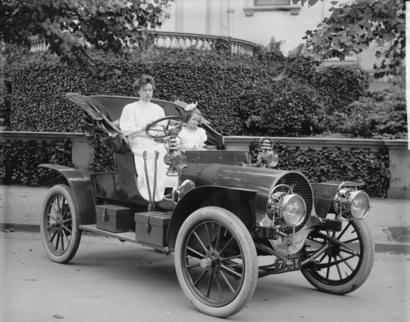
\includegraphics{sample-franklin}
	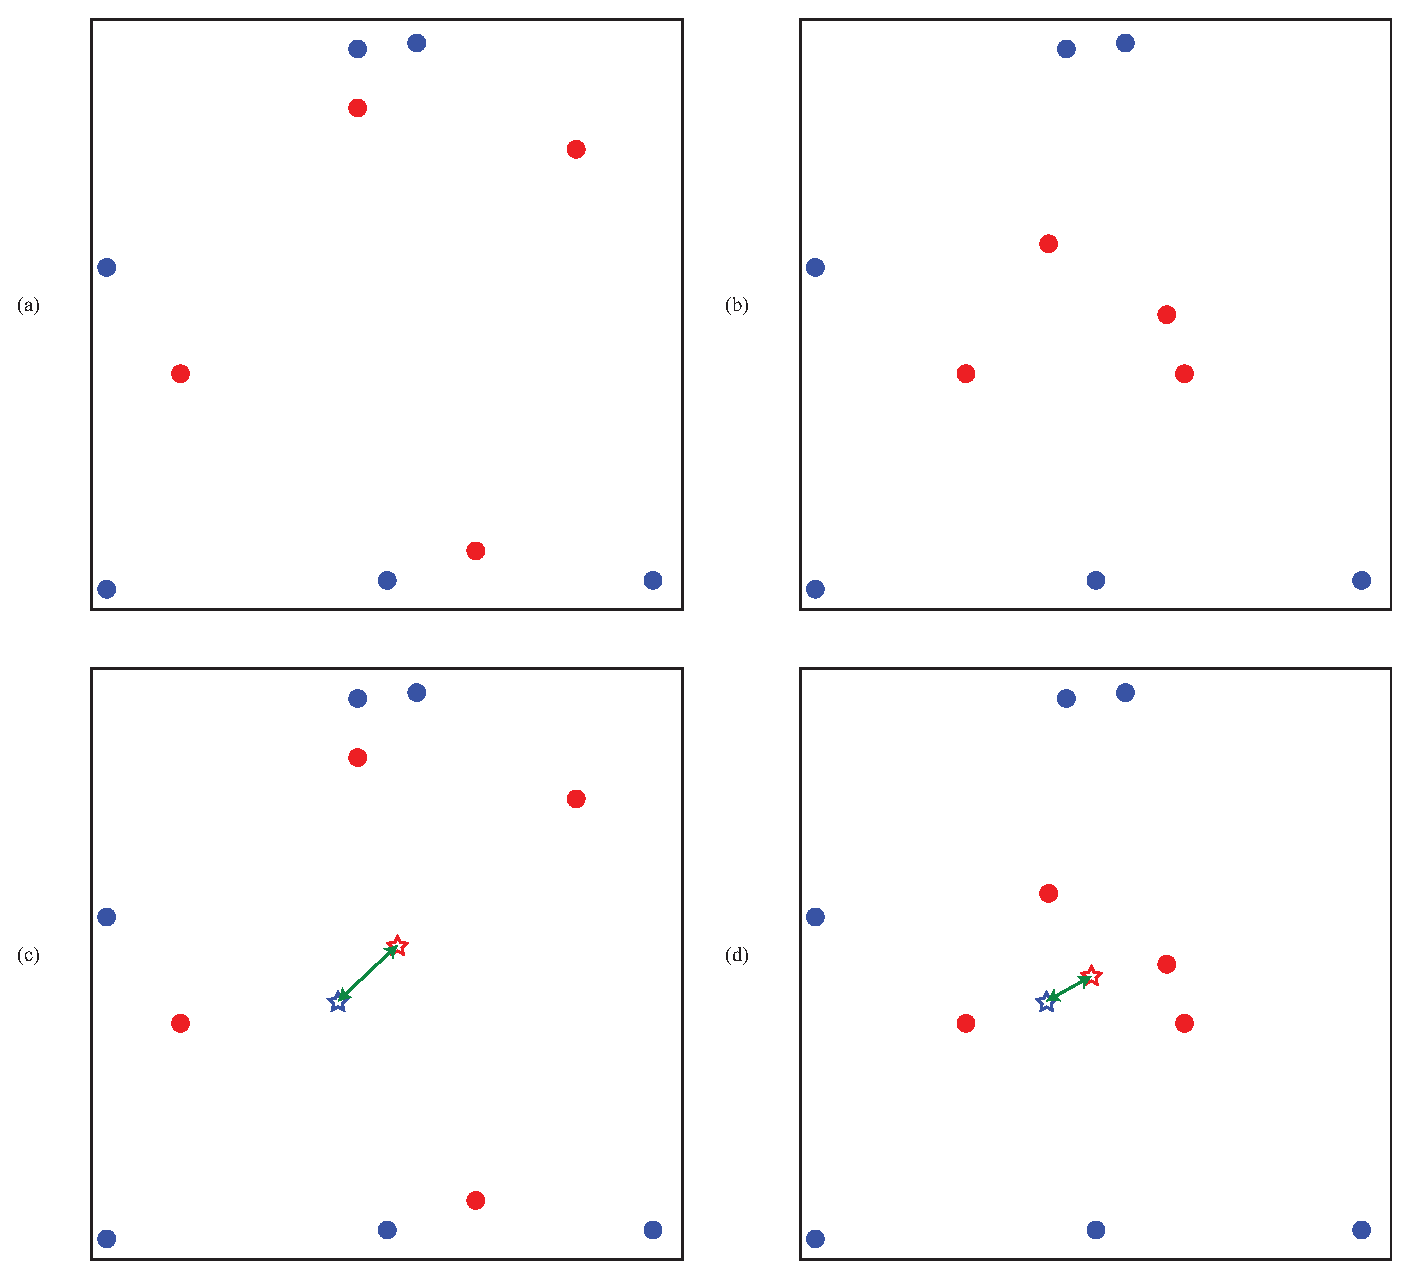
\includegraphics[width=0.8\textwidth]{figs/sarkar_problem-edited}
	\caption{A scenario where sentence averaging method fails. Dots in the figure represent word vectors and are grouped by colours if they are from the same sentence. (a) and (c) shows a scenario where the distance between sentence average vectors are larger than (b) and (d) despite the word vectors being more closely related.}
	\label{fig:sarkar-problem}
\end{figure}

But the sentence average method suffers critically due to its inability in capturing accurate relationship between sentences. This happens due to words in a sentence generally not having similar meaning with each other, instead they express different parts of one whole meaning of a sentence. This makes the words more complementary instead of being similar leading to word vectors being scattered throughout the word vector space. This characteristics makes the sentence average vectors always tending towards the centre and not representing the semantic similarity accurately. An example of this happening is shown in Figure \ref{fig:sarkar-problem} where the distance between the sentence average vectors are being misleading. In the figure, scenario (a) shows two sentence with word vectors very closely corresponding with each other. On the other hand, scenario (b) shows two sentences without any significant word correspondence. The distance between the sentence average vectors  from (a) and (b) are shown in figure (c) and (d) respectively. We can see that the scenario (a) and (c) have a larger distance between sentence average vectors than scenario (b) and (d) despite having more word correspondence. This larger distance makes the Gaussian similarity between the sentences lower due to the inverse exponential nature of the function. The lower similarity leads to the graphical representation being less accurate and thus failing to capture the true semantic relationship within the sentences. This shortcoming of the method has been one of the key motivations for this research.

\section{Methodology}\label{sec:methodology}
The summarization process followed here can be boiled down as two basic steps, grouping all the close sentences together based on their meaning to minimize redundancy and picking one sentence from each group to maximize sentence coverage. To group semantically similar sentences into clusters, we build a sentence similarity graph and perform spectral clustering on it~\cite{roychowdhury-etal-2022-spectral-base}. The sentence similarity graph is produced using a novel sentence similarity calculation algorithm that uses geometric mean of Gaussian similarity between individual word pairs from the two sentences. The Gaussian similarity is calculated using the vector embedding representations of the words. On the other hand, we used TF-IDF scores to pick the highest ranked sentences from a cluster \cite{Akter-2017-tfidf-3, das-2022-tfidf, sarkar-2012-tfidf, sarkar-2012-tfidf-2}. The summarization process followed here involves 4 steps. These are, Pre-processing, Sentence similarity calculation, Clustering and Summary generation. These steps are illustrated in Figure \ref{fig:process-flow-diagram} and further discussed in the following subsections. 
\begin{figure}
	\centering
	%
\begin{tikzpicture}[node distance=1.5cm]

    % Input
    \node (input) [subprocess] {Input Document};

    % Preprocessing
    \node (tokenization) [subprocess, right of=input, yshift=1.5cm, xshift=4cm] {Tokenization};
    \node (stopword) [subprocess, below of=tokenization] {Stopword Removal};
    \node (embedding) [subprocess, below of=stopword] {Word Embedding};

    \node (preprocessbox) [process, fit=(tokenization) (embedding), label=above:Preprocessing] {};

    % Similarity Graph
    \node (summarycalc) [subprocess, right of=stopword, xshift=4.5cm, yshift=.75cm] {Sentence Similarity Calculation};
    \node (affinitymatrix) [subprocess, below of=summarycalc] {Building Affinity Matrix};

    \node (similaritygraphbox) [process, fit=(summarycalc) (affinitymatrix), label=above:Building Similarity Graph] {};

    % Clustering
    \node (clustering) [subprocess, below of=affinitymatrix, anchor=north, yshift=-1.05cm] {Clustering};

    % Picking best sentence
    \node (picksentence) [subprocess, below of=embedding, anchor=north] {Picking the Best Sentence from Each Cluster};

    % Output
    \node (output) [subprocess, below of=input, yshift=-2.25cm] {Output Summary};

    % Draw arrows
    \draw [arrow] (input) -- (preprocessbox);
    \draw [arrow] (tokenization) -- (stopword);
    \draw [arrow] (stopword) -- (embedding);
    \draw [arrow] (preprocessbox) -- (similaritygraphbox);
    \draw [arrow] (summarycalc) -- (affinitymatrix);
    \draw [arrow] (similaritygraphbox) -- (clustering);
    \draw [arrow] (clustering) -- (picksentence);
    \draw [arrow] (picksentence) -- (output);

\end{tikzpicture}

	%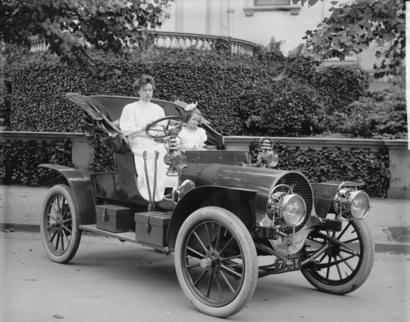
\includegraphics{sample-franklin}
	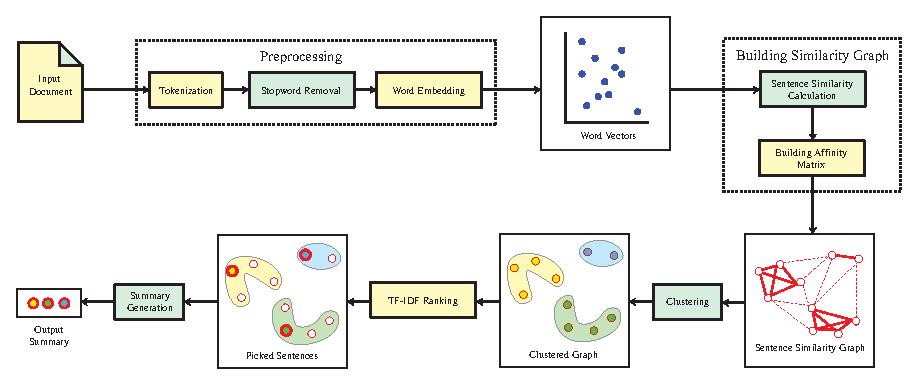
\includegraphics[width=0.8\textwidth]{figs/process-flow-diagram-new}
	\caption{Process Flow Diagram}
	\label{fig:process-flow-diagram}
\end{figure}

\subsection{Preprocessing}\label{subsec:preprocessing}
Preprocessing is the standard process of NLP that transforms raw human language inputs into a format that can be used by a computer algorithm. In this step, the document is transformed into a few set of vectors where each word is represented with a vector, each sentence is represented as a set of vectors and the whole document as a list containing those sets. To achieve this representation, the preprocessing follows three steps. These are tokenization, stop word removal, and word embedding. A very common step in preprocessing, word stemming, isn't used here as the word embedding dataset works best for the whole word instead of the root word. These steps are further discussed below.\\

Tokenization is the step of dividing an input document into sentences and words to transform it into a more usable format. Here, the input document is represented as a list of sentence and the sentences are represented as a list of words. Stop words, such as prepositions and conjunctions, add sentence fluidity but don’t carry significant meaning. Removing these words allows the algorithm to focus on more impactful words. 
%To remove these stop words, we used a list\footnote{\textit{https://www.ranks.nl/stopwords/bengali}} of 363 bengali words. 
Word Embedding is the process of representing words as vector in a vector space. In this vector space, semantically similar words are placed closer together so that the similarity relation between words can be expressed in an abstract mathematical way. 
%We used the FastText dataset\footnote{\textit{https://fasttext.cc/docs/en/crawl-vectors.html}} \cite{grave-etal-2018-fasttext} with 1.47 million Bengali words and their vector representation to achieve this step. 
Each word from the tokenized and filtered list is replaced with their corresponding vectors. If some words aren't present in the dataset, they are considered too rare and thus ignored. Following these steps, the input document is transformed into a set of vectors to be used in sentence similarity calculation. 

\subsection{Sentence Similarity Calculation}\label{subsec:sentence-similarity-calculation}
Sentence similarity is the key criteria to build a graphical representation of the semantic relationship in the input document. This graphical representation is expressed via an affinity matrix to cluster the semantically similar sentences. The nodes in the affinity matrix represents the sentences of the input and the edges of the matrix represents the similarity between two sentence. Here, we proposed a novel sentence similarity calculation technique using individual Gaussian similarity of word-pairs to construct an affinity matrix. To calculate the sentence similarity between two sentences, we adhere to the following steps.\\

Firstly, for every word of a sentence, we find its closest counterpart from the other sentence to build a word pair. The Euclidean distance between the vector representation of the word-pairs is defined as the Most Similar Word Distance ($D_{msw}$). The process of calculating the $D_{msw}$ is shown in the Equation \ref{eq:msd}. In this equation, for every word vector $x$, in a sentence $X$, we find the Euclidean distance ( $d(x,y_i)$ ) between the word vectors $x$ and $y_i$ where $y_i$ is a word vector from the sentence $Y$. The lowest possible distance in this set of Euclidean distance is the $D_{msw}$. 
\begin{equation}\label{eq:msd}
	D_{msw}(x,Y) = min(\{d(x,y_i) : y_i \in Y \})
\end{equation}
Then, we calculate the $D_{msw}$ for every word of the two sentences $X$ and $Y$ to make the sentence similarity calculation symmetric. This process is shown in the Equation \ref{eq:mswdset} where $D$ is a set containing all the $D_{msw}$ from both $X$ and $Y$ that would be used in the later steps.
\begin{equation}
	D = \{D_{msw}(x,Y) : x \in X\} \cup \{D_{msw}(y,X) : y \in Y\}
	\label{eq:mswdset}
\end{equation}
After this, the word similarity between the word pairs is calculated to get the degree of correspondence between the two sentences. Here, the word similarity is calculated using Gaussian kernel function for the elements of the set $D$; Gaussian kernel functions provides a smooth, flexible and most representative similarity between two vectors \cite{babud-1986-gaussian}. The process of calculating word similarity ($W_{sim}$) is given in the Equation \ref{eq:wsim}. In this equation, for every element $D_i$ in set $D$, we calculate the Gaussian similarity to obtain word similarity. In the formula for Gaussian similarity, $\sigma$ denotes the standard deviation that can be used as a control variable. The standard deviation represents the blurring effect of the kernel function. A lower value for $\sigma$ represents a high noise sensitivity of the function \cite{babud-1986-gaussian}. The value of sigma was fine-tuned to be $5\times10^{-11}$ which gives the best similarity measurement. The process of fine-tuning is described in the experimentation section (section \ref{subsubsec:sigma}). 
\begin{equation}\label{eq:wsim}
	W_{sim} = \{ exp\left(\frac{-D_i^2}{2\sigma^2}\right) : D_i \in D\}
\end{equation}
Finally, the sentence similarity between the two sentences $Sim(X,Y)$ is calculated using geometric mean of the word similarities to construct an affinity matrix. The geometric mean makes the similarity value less prone to effects of outliers thus it makes the calculation more reliable. This process is shown in the Equation \ref{eq:sent_sim}; the geometric mean of each $w_{sim}$ value for the two sentences is simplified in the Equation \ref{eq:sent_sim} to make the calculation process more computation friendly. 
\begin{equation}\label{eq:sent_sim}
	\begin{split}
		Sim(X,Y)
		&=  \left(
		\prod_{i=1}^nW_{Sim_i}
		\right)^{\frac{1}{n}}\\
		&=  \left(
		e^{\frac{-D_1^2}{2\sigma^2}}\cdot
		e^{\frac{-D_2^2}{2\sigma^2}}\cdot
		\ldots \cdot
		e^{\frac{-D_n^2}{2\sigma^2}}
		\right)^\frac{1}{n}\\
		&=  exp\left(
		-\frac{D_1^2+D_2^2+\ldots+D_n^2}{2n\sigma^2}
		\right)\\
		&=  exp\left(
		-\frac{\sum_{i=1}^nD_i^2}{2n\sigma^2}
		\right)
	\end{split}
\end{equation}
By following steps described above, we get a similarity value for two sentences. This value solves the lack of local word correspondence problem faced by the word averaging based similarity calculation method \cite{roychowdhury-etal-2022-spectral-base}. Figure \ref{fig:msd} demonstrates the merit of the method claimed above. Figure \ref{fig:msd} 
%follows up the scenario from the Figure \ref{fig:sarkar-problem} to 
shows that the proposed method can solve the local word correspondence problem faced by word averaging method. In the figure, the scenario \ref{fig:msd}(a) has a set of smaller $D_{msw}$ than the scenario \ref{fig:msd}(b). Having smaller $D_{msw}$ makes the individual word similarities $W_{sim}$ larger due to the nature of Gaussian kernel function. These values would result in a higher sentence similarity for the sentences in the scenario \ref{fig:msd}(a) than in the scenario \ref{fig:msd}(b). This solved the problem showed in the Figure \ref{fig:sarkar-problem} where the scenario \ref{fig:sarkar-problem}(a) has a larger sentence average distance than \ref{fig:sarkar-problem}(b) resulting in \ref{fig:sarkar-problem}(a) having a smaller sentence similarity than \ref{fig:sarkar-problem}(b).\\

The whole process of sentence similarity calculation is shown in the Algorithm \ref{alg:similarity}. In this algorithm, we calculate an affinity matrix using the input word vector list. We took the most similar word distance $D_{msw}$ in line 8--13 and 18--23 for each word (line 7 and 17) of a sentence pair (line 3 and 6). Sum of $D^2$ from Equation \ref{eq:sent_sim} is calculated in the lines 14 and 24 to be used in the calculation of sentence similarity (line 27). The similarity is used to construct an affinity matrix $A$ (line 28).
\begin{figure}
	\centering
	%\begin{tikzpicture}[scale=0.00125\textwidth]

    \def\xleft{2};
    \def\xright{14};
    % Draw quarters
    \draw (\xleft,0) rectangle (\xleft+10,10);
    \draw (\xright,0) rectangle (\xright+10,10);

    % Add labels
    \node at (0.95,5.15) {(a)};
    \node at (12.95,5.15) {(b)};

    %set a
    \def\aax{0.25};\def\aay{0.35};
    \def\abx{0.25};\def\aby{5.8};
    \def\acx{5};\def\acy{0.5};
    \def\adx{4.5};\def\ady{9.5};
    \def\aex{5.5};\def\aey{9.6};
    \def\afx{9.5};\def\afy{0.5};
    %set b
    \def\bax{1.5};\def\bay{4};
    \def\bbx{4.5};\def\bby{8.5};
    \def\bcx{6.5};\def\bcy{1};
    \def\bdx{8.2};\def\bdy{7.8};
    %set c
    \def\cax{2.8};\def\cay{4};
    \def\cbx{4.2};\def\cby{6.2};
    \def\ccx{6.2};\def\ccy{5};
    \def\cdx{6.5};\def\cdy{4};



    %set a at a
    \fill[blue] (\xleft+\aax,\aay) circle(.15);
    \fill[blue] (\xleft+\abx,\aby) circle(.15);
    \fill[blue] (\xleft+\acx,\acy) circle(.15);
    \fill[blue] (\xleft+\adx,\ady) circle(.15);
    \fill[blue] (\xleft+\aex,\aey) circle(.15);
    \fill[blue] (\xleft+\afx,\afy) circle(.15);
    %set a at b
    \fill[blue] (\xright+\aax,\aay) circle(.15);
    \fill[blue] (\xright+\abx,\aby) circle(.15);
    \fill[blue] (\xright+\acx,\acy) circle(.15);
    \fill[blue] (\xright+\adx,\ady) circle(.15);
    \fill[blue] (\xright+\aex,\aey) circle(.15);
    \fill[blue] (\xright+\afx,\afy) circle(.15);

     %set b at a
    \fill[red] (\xleft+\bax,\bay) circle(.15);
    \fill[red] (\xleft+\bbx,\bby) circle(.15);
    \fill[red] (\xleft+\bcx,\bcy) circle(.15);
    \fill[red] (\xleft+\bdx,\bdy) circle(.15);

     %set c at b
    \fill[red] (\xright+\cax,\cay) circle(.15);
    \fill[red] (\xright+\cbx,\cby) circle(.15);
    \fill[red] (\xright+\ccx,\ccy) circle(.15);
    \fill[red] (\xright+\cdx,\cdy) circle(.15);


    %drawing line a
    \draw[-{Latex[length=2mm]},dashed] (\xleft+\aax,\aay) -- (\xleft+\bax,\bay);
    \draw[{Latex[length=2mm]}-{Latex[length=2mm]},dashed] (\xleft+\bax,\bay) -- (\xleft+\abx,\aby);
    \draw[{Latex[length=2mm]}-{Latex[length=2mm]},dashed] (\xleft+\bbx,\bby) -- (\xleft+\adx,\ady);
    \draw[{Latex[length=2mm]}-{Latex[length=2mm]},dashed] (\xleft+\bcx,\bcy) -- (\xleft+\acx,\acy);
    \draw[-{Latex[length=2mm]},dashed] (\xleft+\aex,\aey) -- (\xleft+\bbx,\bby);
    \draw[-{Latex[length=2mm]},dashed] (\xleft+\bdx,\bdy) -- (\xleft+\aex,\aey);
    \draw[-{Latex[length=2mm]},dashed] (\xleft+\afx,\afy) -- (\xleft+\bcx,\bcy);

    %drawing line b
    \draw[{Latex[length=2mm]}-{Latex[length=2mm]},dashed] (\xright+\abx,\aby) -- (\xright+\cax,\cay);
    \draw[{Latex[length=2mm]}-{Latex[length=2mm]},dashed] (\xright+\adx,\ady) -- (\xright+\cbx,\cby);
    \draw[{Latex[length=2mm]}-{Latex[length=2mm]},dashed] (\xright+\cdx,\cdy) -- (\xright+\acx,\acy);
    \draw[-{Latex[length=2mm]},dashed] (\xright+\aax,\aay) -- (\xright+\cax,\cay);
    \draw[-{Latex[length=2mm]},dashed] (\xright+\aex,\aey) -- (\xright+\cbx,\cby);
    \draw[-{Latex[length=2mm]},dashed] (\xright+\ccx,\ccy) -- (\xright+\aex,\aey);
    \draw[-{Latex[length=2mm]},dashed] (\xright+\afx,\afy) -- (\xright+\cdx,\cdy);

\end{tikzpicture}
	%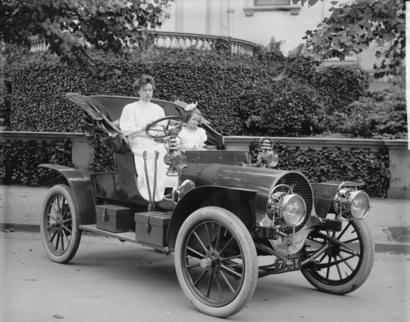
\includegraphics{sample-franklin}
	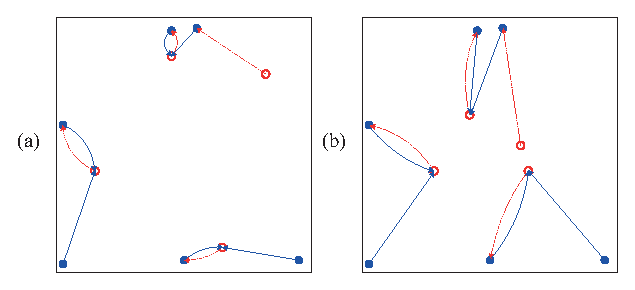
\includegraphics[width=0.8\textwidth]{figs/msd-edited}
	\caption{Local word correspondence of $D_{msw}$ method. Dots in the figure represent word vectors and are coloured with the same colour if they are from the same sentence. Black dashed arrows represent the $D_{msw}$ from its destination word vector. Here, scenario (a) will have larger similarity due to it having smaller $D_{msw}$ than scenario (b)}
	\label{fig:msd}
\end{figure}
\begin{comment}
\begin{algorithm} \caption{Sentence Similarity Calculation} \label{alg:similarity}
	\begin{algorithmic}[1]
		\State $l \gets$ length(WordVectorList)
		\State $A \gets [ [ 0 ] * l ] * l$
		\For{each sentence$_i$ in WordVectorList}
		\State $D_{Square} \gets 0$
		\State n $\gets 0$
		\For{each sentence$_j$ in WordVectorList}
		\For{each word$_i$ in sentence$_i$}
		\State $D_{msw} \gets \infty$
		\For{each word$_j$ in sentence$_j$}
		\If{Distance(word$_i$, word$_j$) $< D_{msw}$}
		\State $D_{msw} \gets$ distance(word$_i$, word$_j$)
		\EndIf
		\EndFor
		\State $D_{Square} \gets D_{Square} + D_{msw}^2$
		\State $n \gets n+1$ 
		\EndFor
		\For{each word$_j$ in sentence$_j$}
		\State $D_{msw} \gets \infty$
		\For{each word$_i$ in sentence$_i$}
		\If{Distance(word$_i$, word$_j$) $< D_{msw}$}
		\State $D_{msw} \gets$ distance(word$_i$, word$_j$)
		\EndIf
		\EndFor
		\State $D_{Square} \gets D_{Square} + D_{msw}^2$
		\State $n \gets n+1$
		\EndFor
		\State similarity $\gets \exp \left( \frac{- D_{Square}}{2 \times n \times \sigma^2} \right)$
		\State $A[i][j] \gets A[j][i] \gets$ similarity
		\EndFor
		\EndFor
		\State \textbf{Return} $A$
	\end{algorithmic}
\end{algorithm}
\end{comment}

\subsection{Clustering}\label{subsec:clustering}
Clustering is a key corner stone of the proposed method where we aim to cluster semantically similar sentences together to divide the input document into multiple topics. Clustering the document minimizes redundancy in the output summary by ignoring multiple sentences from the same topic. For clustering, spectral and DBSCAN methods were considered due to their capability of being able to cluster irregular shapes. However, spectral clustering was found to perform better than DBSCAN because, smaller input documents have lower density which hinders DBSCAN \cite{roychowdhury-etal-2022-spectral-base}.\\

On the contrary, spectral clustering takes the affinity matrix of a graph as input and returns the grouping of graph nodes by transforming the graph into its eigenspace \cite{vonLuxburg-2007-spectral-tutorial}. The following Equation \ref{eq:affinity} shows the process of building an affinity matrix. Here, for every sentence pair $S_i$ and $S_j$, we calculate their sentence similarity and place it in both $A_{ij}$ and $A_{ji}$ of the affinity matrix $A$.
\begin{equation}\label{eq:affinity}
	A_{ij}=A_{ji}=Sim(S_i,S_j)
\end{equation}
The affinity matrix is clustered into a reasonable, $k=\lceil N/5 \rceil$ groups to achieve an output summary. This summary, is short while the sentence groups resulting from clustering is also not too broad.

\subsection{Summary Generation}\label{subsec:summary-generation}
Output summary is generated by selecting one sentence from each cluster achieved in the previous step to minimize topic redundancy and maximize topic coverage. To select one sentence from a cluster, we perform TF-IDF ranking on the sentences inside a cluster and pick the sentence with the highest TF-IDF score. To get the TF-IDF score of a sentence, we take the sum of all TF-IDF values for the words in that sentence. The TF-IDF value for a word is achieved by multiplying how many time the word appeared in the input document (Term Frequency, TF) and the inverse of how many document does the word appear in a corpus (Inverse Document Frequency, IDF). The process of scoring sentences are shown in the Equation \ref{eq:tfidf} where, for each word $W_i$ in a sentence $S$ and a corpus $C$, we calculate the TF-IDF score of a sentence.
\begin{equation}\label{eq:tfidf}
	\text{TFIDF}(S) = \sum_{i=1}^{\text{length}(S)}\text{TF}(W_i) \times \text{IDF}(W_i,C)	
\end{equation}
The sentences with the best TF-IDF score from each clusters are then compiled as the output summary in their order of appearance in the input document to preserve the original flow of information. The process of generating output summary is further expanded in the Algorithm \ref{alg:summary}. After the clustering step (line 2), we took the TF-IDF score (line 7) of each sentence in a cluster (line 6). For each cluster (line 4), we pick the best scoring sentence (line 9). These sentences are then ordered (line 11) and concatenated (line 13--15) to generate the output summary.

\begin{comment}
\begin{algorithm} \caption{Summary Generation} \label{alg:summary}
	\begin{algorithmic}[1]
		\State $k \gets \lceil$ length($A$) / 5 $\rceil$
		\State clusters $\gets$ spectral\_clustering(adjacency = $A$, $k$)
		\State indexes $\gets \{\}$
		\For{each cluster$_i$ in clusters}
		\State TFIDF $\gets \{\}$
		\For{each index in cluster$_i$}
		\State TFIDF.append(tfidf\_sum(sentences[index]))
		\EndFor
		\State indexes.append(indexof(max(TFIDF)))
		\EndFor
		\State sort(indexes)
		\State $S \gets `` "$
		\For{each $i$ in indexes}
		\State $S \gets S +$ sentences[$i$]
		\EndFor
		\State \textbf{Return} $S$
	\end{algorithmic}
\end{algorithm}
\end{comment}

%\subsection{Implementation Details}\label{subsec:implementation}
%The implementation details of the proposed method is provided here for the purpose of reproducibility. While implementing the preprocessing step, we used the nltk package \cite{Bird-2009-nltk} to tokenize the input document. To remove stop words from the tokenized document, we used regex matching in a dataset of 363 Bengali stop words.  

\section{Result}\label{sec:result}
The performance of the proposed method has been compared against three Bengali text summarization methods to evaluate the correctness of generated summaries. The three methods, which have been used as a benchmark, are BenSumm \cite{chowdhury-etal-2021-tfidf-clustering}, LexRank \cite{Erkan-lexRank-2004} and SASbSC \cite{roychowdhury-etal-2022-spectral-base}. All of these methods have been evaluated using four datasets to test the robustness of the model for Bengali text summarization for input from different sources. For evaluation, the Recall-Oriented Understudy for Gisting Evaluation (ROUGE)~\cite{lin-2004-rouge} metric has been used. Details about the models, datasets and evaluation metrics are provided in the following sections.

\subsection{Text Summarization Models}\label{subsec:text-summarization-models}
We implemented Bensumm \cite{chowdhury-etal-2021-tfidf-clustering} and SASbSC \cite{roychowdhury-etal-2022-spectral-base}, two recent Bengali extractive models, and LexRank \cite{Erkan-lexRank-2004}, a popular benchmarking model for extractive text summarization to evaluate the effectiveness of the proposed WSbSC method. These methods are further discussed in the following section.\\

\textbf{WSbSC} is the proposed model for this research. We find the Gaussian similarity for word-pairs from two sentences and take their geometric mean to get the similarity between two sentences. We use the similarity value to perfom spectral clustering to group sentences into groups and extract a representative sentence using TF-IDF score. The extracted sentences are used to generate the output summary which minimizes redundancy and maximizes coverage.\\

\textbf{SASbSC} \cite{roychowdhury-etal-2022-spectral-base} is the first method that introduced the approach of clustering sentences using sentence similarity. However, it uses the average of word vectors in a sentence for calculating similarity. After clustering the sentences based on their similarity, cosine similarity between the average vectors are used to pick the best sentence from a cluster.\\

\textbf{BenSumm} \cite{chowdhury-etal-2021-tfidf-clustering} is another recent research that describes an extractive and an abstractive text summarization technique. We compared the extractive technique with our model to ensure a fair and balanced comparison. Here, similarity matrix is built using TF-IDF which groups the sentences using agglomerative clustering. A Github implementation\footnote{\textit{https://github.com/tafseer-nayeem/BengaliSummarization}} provided by the authors is used in the comparison process.\\

\textbf{LexRank} \cite{Erkan-lexRank-2004} uses a TF-IDF based matrix and Googles PageRank algorithm \cite{page-PageRank-1999} to rank sentences. Then the top ranked sentences are selected and arranged into summary. An implemented version of this method is available as lexrank\footnote{\textit{https://pypi.org/project/lexrank/}} which is used in the comparison process using a large Bengali wikipedia corpus\footnote{\textit{https://www.kaggle.com/datasets/shazol/bangla-wikipedia-corpus}}.

\subsection{Evaluation Datasets}\label{subsec:evaluation-datasets}
We used four evaluation dataset with varying quality, size and source to examine the robustness of the methods being tested. The first dataset is a \textbf{self-curated} extractive dataset that we developed to evaluate the performance of our proposed method. An expert linguistic team of ten members summarized 250 news articles of varying sizes to diversify the dataset. Each article is summarized twice by two different experts to minimize human bias in the summary. In total, 500 different document-summary pairs are present in this dataset. The dataset is publicly available on Github\footnote{\textit{dataset link}} for reproducibility.\\

The second dataset is collected from \textbf{Kaggle} dataset\footnote{\textit{https://www.kaggle.com/datasets/towhidahmedfoysal/bangla-summarization-datasetprothom-alo}} which is a collection of summary-article pair from ``The Daily Prothom Alo" newspaper. The dataset is vast in size however the quality of the summaries are poor. All the articles smaller than 50 characters were discarded from the dataset. The articles with unrelated summaries were also removed from the dataset to improve the quality. After filtering, total 10,204 articles remained, each with two summaries in the dataset.\\

The third dataset we used for evaluation is \textbf{BNLPC} which is a collection of news article summaries \cite{Hque-2015-BNLPC-Dataset}. This was collected from GitHub\footnote{\textit{https://github.com/tafseer-nayeem/BengaliSummarization/tree/main/Dataset/BNLPC/Dataset2}} for experimentation that contains one hundred articles with three different summaries for each article.\\

The fourth dataset is collected from \textbf{Github}\footnote{\textit{https://github.com/Abid-Mahadi/Bangla-Text-summarization-Dataset}}. The dataset contains 200 documents each with two human generated summaries. These documents were collected from several different Bengali news portals. The summaries were generated by linguistic experts which ensures the high quality of the dataset.

\subsection{Evaluation Metrics}\label{subsec:evaluation-metrics}
To evaluate the correctness of generated summaries against human written summaries, ROUGE metric \cite{lin-2004-rouge} is used. The method compares a reference summary with a machine generated summary to evaluate alignment between the two. It uses N-gram-based overlapping to calculate a precision, recall and F-1 score of each summary. The Rouge package\footnote{\textit{https://pypi.org/project/rouge/}} is used to evaluate the proposed models against human generated summaries. The package has three different metrics for comparison of summaries. These are are:

\begin{enumerate}
	\item \textbf{ROUGE-1} uses unigram matching to find how similar two summaries are. It calculates total common characters between the summaries to evaluate the performance. But using this metric also can be misleading as very large texts will share a very high proportion of uni-grams between them.
	
	\item \textbf{ROUGE-2} uses bi-gram matching to find how much similar the two summaries are in a word level. Having more common bigrams between two summaries indicates a deeper syntactic similarity between them. Using this in combination with the ROUGE-1 is a standard practice to evaluate machine generated summaries \cite{wafaa-2021-summary-comprehensive-review}.
	
	\item \textbf{ROUGE-LCS} finds the longest common sub-sequence between two summaries to calculate the rouge scores. It focuses on finding similarity in the flow of information in the sentence level between two summaries.
\end{enumerate}

In this study, we compared the F-1 scores from each of these metrics for the four models.


\subsection{Experimentation}\label{subsec:experimentation}
The proposed model contains three main steps, similarity calculation, clustering and sentence extraction. Each of these steps have different techniques or values that can be experimented on to find the most suited strategy. For sentence similarity calculation, different values for standard deviation ($\sigma$) can be fixed to get the most representative semantic similarity value. Spectral clustering was found to work best for the clustering step through experimentations done by other researchers \cite{roychowdhury-etal-2022-spectral-base}. To extract the best sentence from a cluster, lead extraction and TF-IDF ranking strategies was considered. Thus, experimentations on finding the most suited standard deviation value and sentence extraction was conducted. These experimentations are described in the following sections.

\subsubsection{Fine-tuning Standard Deviation ($\sigma$)}\label{subsubsec:sigma}
Standard deviation ($\sigma$) plays a crucial role for sentence similarity calculation (Equation \ref{eq:sent_sim}). Therefore, to fix the most suited $\sigma$ value sixty-three different values were experimented on. These values ranged from $10^{-12}$ to $10$ on regular intervals. After experimentation, $5\times10^{-11}$ was fixed as the value for $\sigma$ that gives the most representative semantic relation between sentences. The result for fine-tuning process is shown in Figure \ref{fig:sigma-fine-tuning}.
\begin{figure}[]
	\centering
	%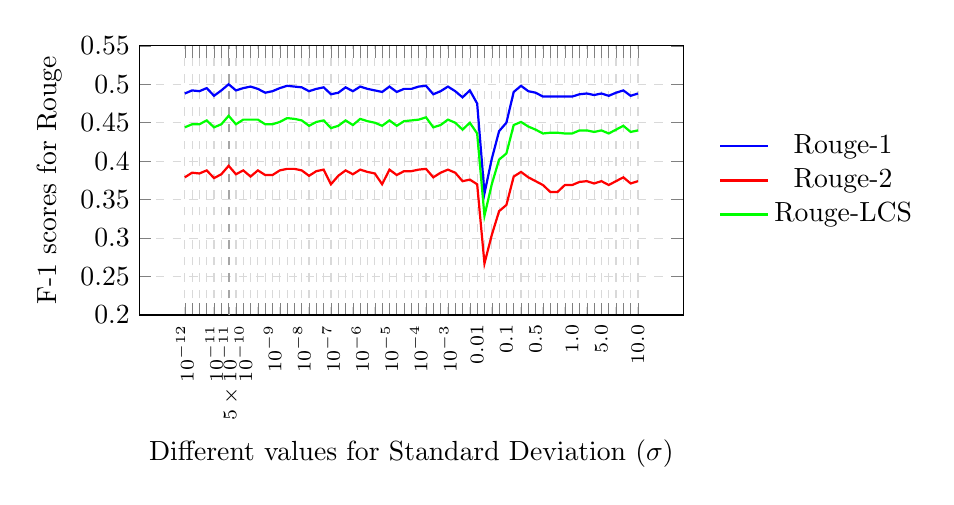
\begin{tikzpicture}
    \begin{axis}[
        width=.7\textwidth,
        height=5cm,
        xlabel={Different values for Standard Deviation ($\sigma$)},
        ylabel={F-1 scores for Rouge},
        ymin=0.2, ymax=0.55,
        xtick={1,2,...,63}, % Original 63 ticks
        xticklabels={ $10^{-12}$, , , , $10^{-11}$, ,$5\times10^{-11}$, , $10^{-10}$, , , , $10^{-9}$, , , , $10^{-8}$, , , ,
                     $10^{-7}$, , , , $10^{-6}$, , , , $10^{-5}$, , , , $10^{-4}$, , , ,
                     $10^{-3}$, , , , $0.01$, , , , $0.1$, , , , $0.5$, , , ,
                      , $1.0$, , , , $5.0$, , , , ,$10.0$}, % Show 1 in every 4 labels
        xticklabel style={rotate=90, anchor=east, font=\scriptsize}, % Rotate labels 90 degrees
        legend style={at={(1.05,0.5)}, anchor=west, draw=none}, % Move legend outside, remove border
        extra x ticks={7}, % Add extra tick for 7th position
        extra x tick style={grid=major, major grid style={gray!70, thick}}, % Style for the highlighted tic
        extra x tick labels={},
        grid=major,
        grid style={dashed,gray!30},
        ytick={0.20, 0.25, 0.30, 0.35, 0.40, 0.45, 0.50, 0.55}, % Y-axis ticks
        cycle list name=color list,
    ]

    % Dummy data for Column 1
    \addplot[color=blue, thick] coordinates {
        (1, 0.488)
        (2, 0.492)
        (3, 0.491)
        (4, 0.495)
        (5, 0.485)
        (6, 0.492)
        (7, 0.500)
        (8, 0.492)
        (9, 0.495)
        (10, 0.497)
        (11, 0.494)
        (12, 0.489)
        (13, 0.491)
        (14, 0.495)
        (15, 0.498)
        (16, 0.497)
        (17, 0.496)
        (18, 0.491)
        (19, 0.494)
        (20, 0.496)
        (21, 0.487)
        (22, 0.489)
        (23, 0.496)
        (24, 0.491)
        (25, 0.497)
        (26, 0.494)
        (27, 0.492)
        (28, 0.490)
        (29, 0.497)
        (30, 0.490)
        (31, 0.494)
        (32, 0.494)
        (33, 0.497)
        (34, 0.498)
        (35, 0.487)
        (36, 0.491)
        (37, 0.497)
        (38, 0.491)
        (39, 0.483)
        (40, 0.492)
        (41, 0.475)
        (42, 0.358)
        (43, 0.403)
        (44, 0.439)
        (45, 0.450)
        (46, 0.490)
        (47, 0.498)
        (48, 0.491)
        (49, 0.489)
        (50, 0.484)
        (51, 0.484)
        (52, 0.484)
        (53, 0.484)
        (54, 0.484)
        (55, 0.487)
        (56, 0.488)
        (57, 0.486)
        (58, 0.488)
        (59, 0.485)
        (60, 0.489)
        (61, 0.492)
        (62, 0.485)
        (63, 0.488)
    };
    \addlegendentry{Rouge-1}

    % Dummy data for Column 2
    \addplot[color=red, thick] coordinates {
        (1, 0.379)
        (2, 0.385)
        (3, 0.384)
        (4, 0.388)
        (5, 0.378)
        (6, 0.383)
        (7, 0.394)
        (8, 0.383)
        (9, 0.388)
        (10, 0.380)
        (11, 0.388)
        (12, 0.382)
        (13, 0.382)
        (14, 0.388)
        (15, 0.390)
        (16, 0.390)
        (17, 0.388)
        (18, 0.381)
        (19, 0.387)
        (20, 0.389)
        (21, 0.370)
        (22, 0.381)
        (23, 0.388)
        (24, 0.383)
        (25, 0.389)
        (26, 0.386)
        (27, 0.384)
        (28, 0.370)
        (29, 0.389)
        (30, 0.382)
        (31, 0.387)
        (32, 0.387)
        (33, 0.389)
        (34, 0.390)
        (35, 0.379)
        (36, 0.385)
        (37, 0.389)
        (38, 0.385)
        (39, 0.374)
        (40, 0.376)
        (41, 0.370)
        (42, 0.267)
        (43, 0.304)
        (44, 0.335)
        (45, 0.343)
        (46, 0.380)
        (47, 0.386)
        (48, 0.379)
        (49, 0.374)
        (50, 0.369)
        (51, 0.360)
        (52, 0.360)
        (53, 0.369)
        (54, 0.369)
        (55, 0.373)
        (56, 0.374)
        (57, 0.371)
        (58, 0.374)
        (59, 0.369)
        (60, 0.374)
        (61, 0.379)
        (62, 0.371)
        (63, 0.374)
    };
    \addlegendentry{Rouge-2}

    % Dummy data for Column 3
    \addplot[color=green, thick] coordinates {
        (1, 0.444)
        (2, 0.448)
        (3, 0.448)
        (4, 0.453)
        (5, 0.444)
        (6, 0.448)
        (7, 0.459)
        (8, 0.448)
        (9, 0.454)
        (10, 0.454)
        (11, 0.454)
        (12, 0.448)
        (13, 0.448)
        (14, 0.451)
        (15, 0.456)
        (16, 0.455)
        (17, 0.453)
        (18, 0.446)
        (19, 0.451)
        (20, 0.453)
        (21, 0.443)
        (22, 0.446)
        (23, 0.453)
        (24, 0.447)
        (25, 0.455)
        (26, 0.452)
        (27, 0.450)
        (28, 0.446)
        (29, 0.453)
        (30, 0.446)
        (31, 0.452)
        (32, 0.453)
        (33, 0.454)
        (34, 0.457)
        (35, 0.444)
        (36, 0.447)
        (37, 0.454)
        (38, 0.450)
        (39, 0.441)
        (40, 0.450)
        (41, 0.436)
        (42, 0.329)
        (43, 0.370)
        (44, 0.402)
        (45, 0.410)
        (46, 0.447)
        (47, 0.451)
        (48, 0.445)
        (49, 0.441)
        (50, 0.436)
        (51, 0.437)
        (52, 0.437)
        (53, 0.436)
        (54, 0.436)
        (55, 0.440)
        (56, 0.440)
        (57, 0.438)
        (58, 0.440)
        (59, 0.436)
        (60, 0.441)
        (61, 0.446)
        (62, 0.438)
        (63, 0.440)
    };
    \addlegendentry{Rouge-LCS}

    \end{axis}
\end{tikzpicture}
	%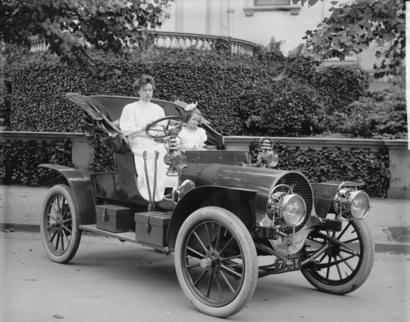
\includegraphics{sample-franklin}
	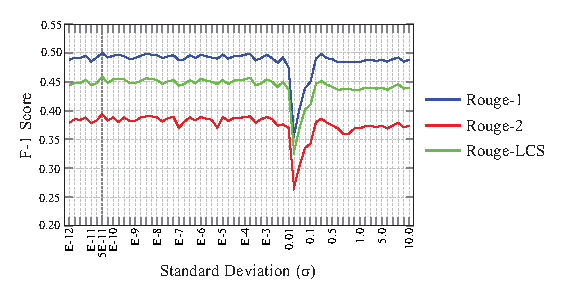
\includegraphics[width=0.8\textwidth]{figs/fine-tuning-edited}
	\caption{Fine-tuning for different standard deviation~($\sigma$)~values}
	\label{fig:sigma-fine-tuning}
\end{figure}
\subsubsection{Different Sentence Extraction Techniques Inside Clusters} \label{subsubsec:different-ranking-techniques-inside-clusters}
We implemented two sentence extraction methods to pick the most representative sentence from each cluster. Firstly, the lead extraction method is used to select the sentence that appears first in the input document. Because, generally the earlier sentences in an input contain more information on the context of the input document. Secondly, extracting sentences based on their TF-IDF score was also experimented on. In Table \ref{tab:ranking}, the TF-IDF ranking is shown to performs better than the lead extraction method.
\begin{table}[]
	\centering
	\begin{tabular}{lccc}\hline
		Method      	& Rouge-1       & Rouge-2       & Rouge-LCS     \\\hline
		Lead extraction	& 0.47          & 0.36          & 0.43          \\
		TF-IDF ranking	& \textbf{0.50} & \textbf{0.40} & \textbf{0.46} \\\hline
	\end{tabular}
	\caption{Comparison of Result of different ranking techniques}
	\label{tab:ranking}
\end{table}
\subsection{Comparison}\label{subsec:comparison}
The performance of the proposed method (WSbSC) is compared with BenSumm \cite{chowdhury-etal-2021-tfidf-clustering}, SASbSC \cite{roychowdhury-etal-2022-spectral-base} and LexRank \cite{Erkan-lexRank-2004} on four datasets (Self-Curated (SC), Kaggle, BNLPC, Github) using the average F-1 score for three ROUGE metrics (Rouge-1, Rouge-2, Rouge-LCS). The comparative results of this evaluation are shown in Table \ref{tab:result_comparison-1} where our proposed model performs 11.9\%, 24.1\% and 16.2\% better than SASbSC in Rouge-1, Rouge-2 and Rouge-LCS respectively on the self-curated dataset. It performs 68.9\%, 95.4\% and 84.6\% better in Rouge-1, Rouge-2 and Rouge-LCS respectively than BenSumm on the Kaggle dataset. It also performs 3\% and 2.6\% better in Rouge-2 and Rouge-LCS respectively and ties in Rouge-1 with SASbSC using the BNLPC dataset. It performs 58\%, 86.4\%, and 67.9\% better in Rouge-1, Rouge-2 and Rouge-LCS respectively than BenSumm on the Github dataset.\\

\begin{table}[]
	\centering
	\begin{tabular}{llccc} \hline
		Dataset 		& Model                                                & Rouge-1       & Rouge-2       & Rouge-LCS     \\\hline
		Self-curated	& WSbSC (Proposed)                                     & \textbf{0.47} & \textbf{0.36} & \textbf{0.43} \\
		& BenSumm \cite{chowdhury-etal-2021-tfidf-clustering}  & 0.41          & 0.29          & 0.36          \\
		& SASbSC \cite{roychowdhury-etal-2022-spectral-base}   & 0.42          & 0.29          & 0.37          \\
		& LexRank \cite{Erkan-lexRank-2004}                    & 0.22          & 0.14          & 0.20          \\\hline
		Kaggle			& WSbSC (Proposed)                                     & \textbf{0.49} & \textbf{0.43} & \textbf{0.48} \\
		& BenSumm \cite{chowdhury-etal-2021-tfidf-clustering}  & 0.29          & 0.22          & 0.26          \\
		& SASbSC \cite{roychowdhury-etal-2022-spectral-base}   & 0.23          & 0.12          & 0.18          \\
		& LexRank \cite{Erkan-lexRank-2004}                    & 0.24          & 0.16          & 0.22          \\\hline
		BNLPC 			& WSbSC (Proposed)                                     & \textbf{0.41} & \textbf{0.34} & \textbf{0.40} \\
		& BenSumm \cite{chowdhury-etal-2021-tfidf-clustering}  & 0.36          & 0.28          & 0.34          \\
		& SASbSC \cite{roychowdhury-etal-2022-spectral-base}   & \textbf{0.41} & 0.33          & 0.39          \\
		& LexRank \cite{Erkan-lexRank-2004}                    & 0.26          & 0.19          & 0.24          \\\hline
		Github          & WSbSC (Proposed)                                     & \textbf{0.49} & \textbf{0.41} & \textbf{0.47} \\
		& BenSumm \cite{chowdhury-etal-2021-tfidf-clustering}  & 0.31          & 0.22          & 0.28          \\
		& SASbSC \cite{roychowdhury-etal-2022-spectral-base}   & 0.30          & 0.18          & 0.24          \\
		& LexRank \cite{Erkan-lexRank-2004}                    & 0.22          & 0.14          & 0.20          \\\hline
	\end{tabular}
	\caption{Comparison of average Rouge scores between graph based extractive summarization models on 4 datasets}
	\label{tab:result_comparison-1}
\end{table}
\begin{figure}[]
	\centering
%	\scalebox{0.55}{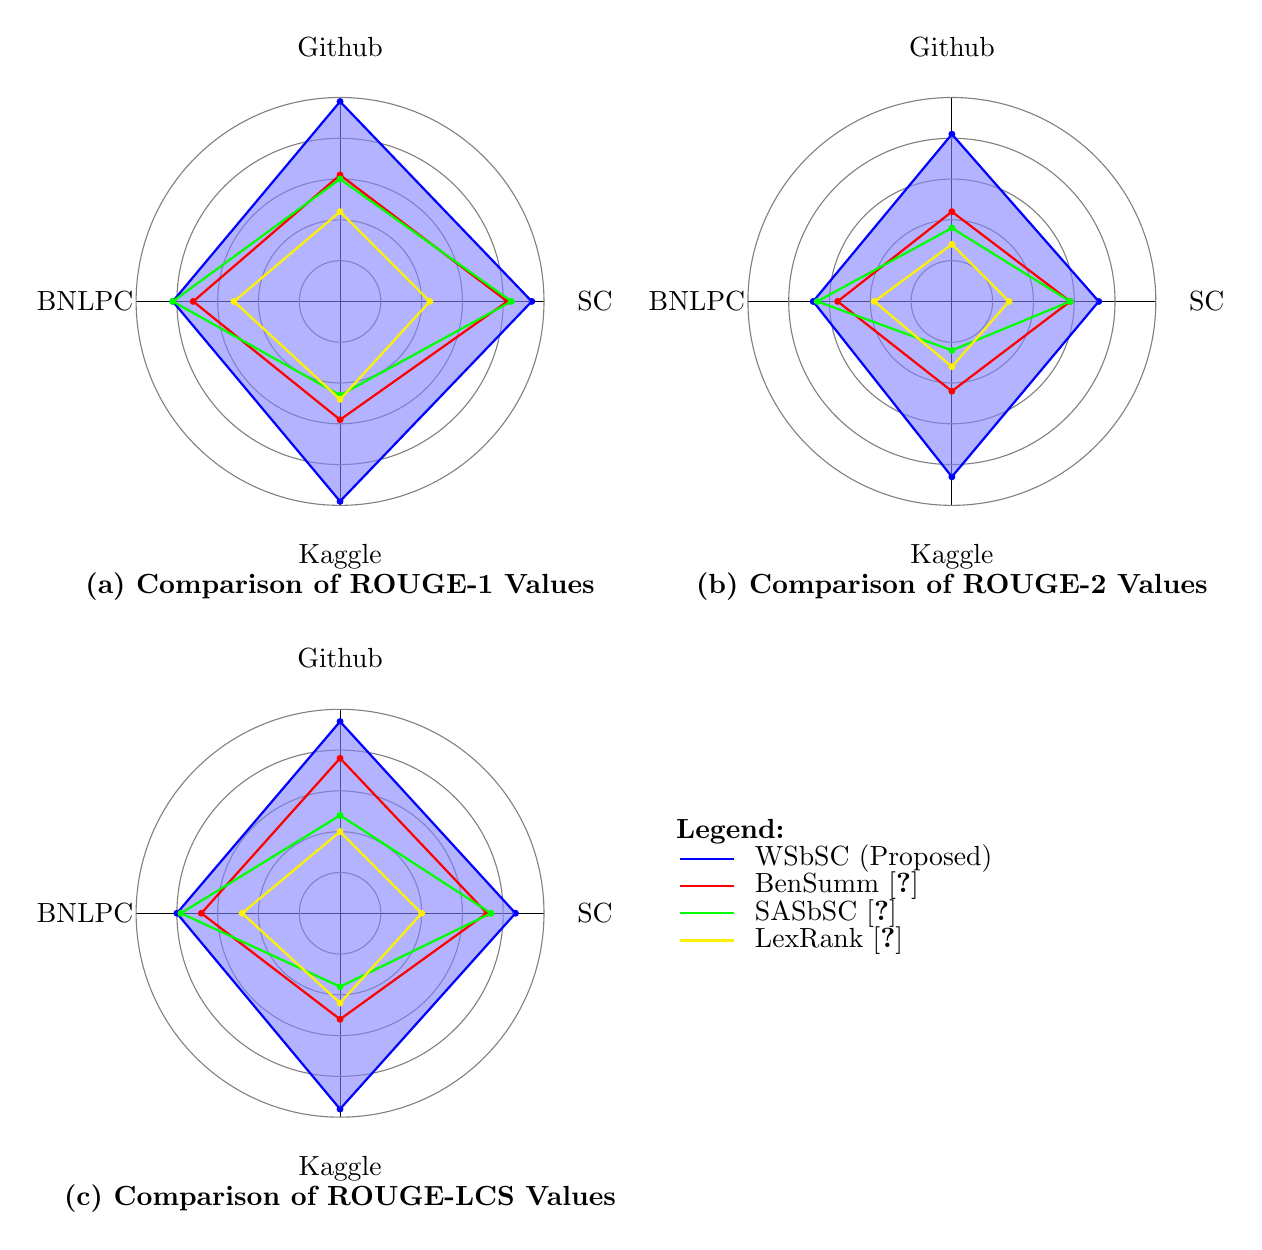
\begin{tikzpicture}[scale=0.0025*\textwidth]
    % Define the number of axes (dimensions)
    \def\n{4}
    % Define the names of the features
    \def\features{{"SC", "Kaggle", "BNLPC", "Github"}}
    % Define the maximum value
    \def\maxvalue{5}

    % Define values for three different radar charts
    \def\valuesAW{{4.7, 4.9, 4.1, 4.9}}
    \def\valuesAB{{4.1, 2.9, 3.6, 3.1}}
    \def\valuesAS{{4.2, 2.3, 4.1, 3.0}}
    \def\valuesAL{{2.2, 2.4, 2.6, 2.2}}

    \def\valuesBW{{3.6, 4.3, 3.4, 4.1}}
    \def\valuesBB{{2.9, 2.2, 2.8, 2.2}}
    \def\valuesBS{{2.9, 1.2, 3.3, 1.8}}
    \def\valuesBL{{1.4, 1.6, 1.9, 1.4}}

    \def\valuesCW{{4.3, 4.8, 4.0, 4.7}}
    \def\valuesCB{{3.6, 2.6, 3.4, 3.8}}
    \def\valuesCS{{3.7, 1.8, 3.9, 2.4}}
    \def\valuesCL{{2.0, 2.2, 2.4, 2.0}}

    % First Radar Chart (Top-left quarter)
    \begin{scope}[xshift=-5cm, yshift=5cm, scale=0.6]
        %write the dataset labels
        \foreach \i in {1,...,\n} {
            \draw (90-\i*360/\n:5) -- (0,0);
            \node at (90-\i*360/\n:6.25) {\pgfmathparse{\features[\i-1]}\pgfmathresult};
        }
        %draw the circle
        \node at (90-2*360/4:7){\textbf{(a) Comparison of ROUGE-1 Values}};
        \foreach \j in {1,...,\maxvalue} {
            \draw[gray, thin] (0,0) circle (\j);
        }

        %draw wsbsc
        \foreach \i [evaluate={\angle=90-\i*360/\n; \valueAW=\valuesAW[\i-1];}] in {1,...,\n} {
            \coordinate (PA\i) at (\angle:\valueAW);
            \filldraw[blue] (PA\i) circle (2pt);
        }
        \fill[blue!50, opacity=0.6] (PA1) -- (PA2) -- (PA3) -- (PA4) -- cycle;
        \foreach \i in {1,...,\n} {
            \pgfmathtruncatemacro{\nexti}{mod(\i,\n)+1}
%                    \draw [thick, cyan] plot [smooth, tension=2] coordinates { (PA\i) (PA\nexti)};
            \draw[thick, blue] (PA\i) -- (PA\nexti);
        }
%                \draw [thick,cyan] plot [smooth cycle, tension=1] coordinates { (PA1) (PA2) (PA3) (PA4)};

        %draw bensumm
        \foreach \i [evaluate={\angle=90-\i*360/\n; \valueAB=\valuesAB[\i-1];}] in {1,...,\n} {
            \coordinate (PB\i) at (\angle:\valueAB);
            \filldraw[red] (PB\i) circle (2pt);
        }
        \foreach \i in {1,...,\n} {
            \pgfmathtruncatemacro{\nexti}{mod(\i,\n)+1}
            \draw[thick, red] (PB\i) -- (PB\nexti);
        }

%                draw sasbsc
        \foreach \i [evaluate={\angle=90-\i*360/\n; \valueAS=\valuesAS[\i-1];}] in {1,...,\n} {
            \coordinate (PC\i) at (\angle:\valueAS);
            \filldraw[green] (PC\i) circle (2pt);
        }
        \foreach \i in {1,...,\n} {
            \pgfmathtruncatemacro{\nexti}{mod(\i,\n)+1}
            \draw[thick, green] (PC\i) -- (PC\nexti);
        }

        %draw lexrank
        \foreach \i [evaluate={\angle=90-\i*360/\n; \valueAL=\valuesAL[\i-1];}] in {1,...,\n} {
            \coordinate (PD\i) at (\angle:\valueAL);
            \filldraw[yellow] (PD\i) circle (2pt);
        }
        \foreach \i in {1,...,\n} {
            \pgfmathtruncatemacro{\nexti}{mod(\i,\n)+1}
            \draw[thick, yellow] (PD\i) -- (PD\nexti);
        }
    \end{scope}

    % Second Radar Chart (Top-right quarter)
    \begin{scope}[xshift=4cm, yshift=5cm, scale=0.6]
        \foreach \i in {1,...,\n} {
            \draw (90-\i*360/\n:5) -- (0,0);
            \node at (90-\i*360/\n:6.25) {\pgfmathparse{\features[\i-1]}\pgfmathresult};
        }
        \node at (90-2*360/4:7){\textbf{(b) Comparison of ROUGE-2 Values}};
        \foreach \j in {1,...,\maxvalue} {
            \draw[gray, thin] (0,0) circle (\j);
        }

        \foreach \i [evaluate={\angle=90-\i*360/\n; \valueBW=\valuesBW[\i-1];}] in {1,...,\n} {
            \coordinate (PA\i) at (\angle:\valueBW);
            \filldraw[blue] (PA\i) circle (2pt);
        }
        \fill[blue!50, opacity=0.6] (PA1) -- (PA2) -- (PA3) -- (PA4) -- cycle;
        \foreach \i in {1,...,\n} {
            \pgfmathtruncatemacro{\nexti}{mod(\i,\n)+1}
            \draw[thick, blue] (PA\i) -- (PA\nexti);
        }

        \foreach \i [evaluate={\angle=90-\i*360/\n; \valueBB=\valuesBB[\i-1];}] in {1,...,\n} {
            \coordinate (PB\i) at (\angle:\valueBB);
            \filldraw[red] (PB\i) circle (2pt);
        }
        \foreach \i in {1,...,\n} {
            \pgfmathtruncatemacro{\nexti}{mod(\i,\n)+1}
            \draw[thick, red] (PB\i) -- (PB\nexti);
        }

        \foreach \i [evaluate={\angle=90-\i*360/\n; \valueBS=\valuesBS[\i-1];}] in {1,...,\n} {
            \coordinate (PC\i) at (\angle:\valueBS);
            \filldraw[green] (PC\i) circle (2pt);
        }
        \foreach \i in {1,...,\n} {
            \pgfmathtruncatemacro{\nexti}{mod(\i,\n)+1}
            \draw[thick, green] (PC\i) -- (PC\nexti);
        }

        \foreach \i [evaluate={\angle=90-\i*360/\n; \valueBL=\valuesBL[\i-1];}] in {1,...,\n} {
            \coordinate (PD\i) at (\angle:\valueBL);
            \filldraw[yellow] (PD\i) circle (2pt);
        }
        \foreach \i in {1,...,\n} {
            \pgfmathtruncatemacro{\nexti}{mod(\i,\n)+1}
            \draw[thick, yellow] (PD\i) -- (PD\nexti);
        }
    \end{scope}

    % Third Radar Chart (Bottom-left quarter)
    \begin{scope}[xshift=-5cm, yshift=-4cm, scale=0.6]
        \foreach \i in {1,...,\n} {
            \draw (90-\i*360/\n:5) -- (0,0);
            \node at (90-\i*360/\n:6.25) {\pgfmathparse{\features[\i-1]}\pgfmathresult};
        }
        \node at (90-2*360/4:7){\textbf{(c) Comparison of ROUGE-LCS Values}};
        \foreach \j in {1,...,\maxvalue} {
            \draw[gray, thin] (0,0) circle (\j);
        }

        \foreach \i [evaluate={\angle=90-\i*360/\n; \valueCW=\valuesCW[\i-1];}] in {1,...,\n} {
            \coordinate (PA\i) at (\angle:\valueCW);
            \filldraw[blue] (PA\i) circle (2pt);
        }
        \fill[blue!50, opacity=0.6] (PA1) -- (PA2) -- (PA3) -- (PA4) -- cycle;
        \foreach \i in {1,...,\n} {
            \pgfmathtruncatemacro{\nexti}{mod(\i,\n)+1}
            \draw[thick, blue] (PA\i) -- (PA\nexti);
        }

        \foreach \i [evaluate={\angle=90-\i*360/\n; \valueCB=\valuesCB[\i-1];}] in {1,...,\n} {
            \coordinate (PB\i) at (\angle:\valueCB);
            \filldraw[red] (PB\i) circle (2pt);
        }
        \foreach \i in {1,...,\n} {
            \pgfmathtruncatemacro{\nexti}{mod(\i,\n)+1}
            \draw[thick, red] (PB\i) -- (PB\nexti);
        }

        \foreach \i [evaluate={\angle=90-\i*360/\n; \valueCS=\valuesCS[\i-1];}] in {1,...,\n} {
            \coordinate (PC\i) at (\angle:\valueCS);
            \filldraw[green] (PC\i) circle (2pt);
        }
        \foreach \i in {1,...,\n} {
            \pgfmathtruncatemacro{\nexti}{mod(\i,\n)+1}
            \draw[thick, green] (PC\i) -- (PC\nexti);
        }

        \foreach \i [evaluate={\angle=90-\i*360/\n; \valueCL=\valuesCL[\i-1];}] in {1,...,\n} {
            \coordinate (PD\i) at (\angle:\valueCL);
            \filldraw[yellow] (PD\i) circle (2pt);
        }
        \foreach \i in {1,...,\n} {
            \pgfmathtruncatemacro{\nexti}{mod(\i,\n)+1}
            \draw[thick, yellow] (PD\i) -- (PD\nexti);
        }
    \end{scope}

    % Legend (Bottom-right quarter)
    \begin{scope}[xshift=4cm, yshift=-4cm, scale=0.8]
        \node[anchor=west] at (-5.25, 1.5) {\textbf{Legend:}};
        \draw[thick, blue] (-5, 1) -- (-4, 1);
        \node[anchor=west] at (-3.8, 1) {WSbSC (Proposed)};

        \draw[thick, red] (-5, 0.5) -- (-4, 0.5);
        \node[anchor=west] at (-3.8, 0.5) {BenSumm~\cite{chowdhury-etal-2021-tfidf-clustering}};

        \draw[thick, green] (-5, 0) -- (-4, 0);
        \node[anchor=west] at (-3.8, 0) {SASbSC~\cite{roychowdhury-etal-2022-spectral-base}};

        \draw[thick, yellow] (-5, -0.5) -- (-4, -0.5);
        \node[anchor=west] at (-3.8, -0.5) {LexRank~\cite{Erkan-lexRank-2004}};
    \end{scope}
\end{tikzpicture}}
	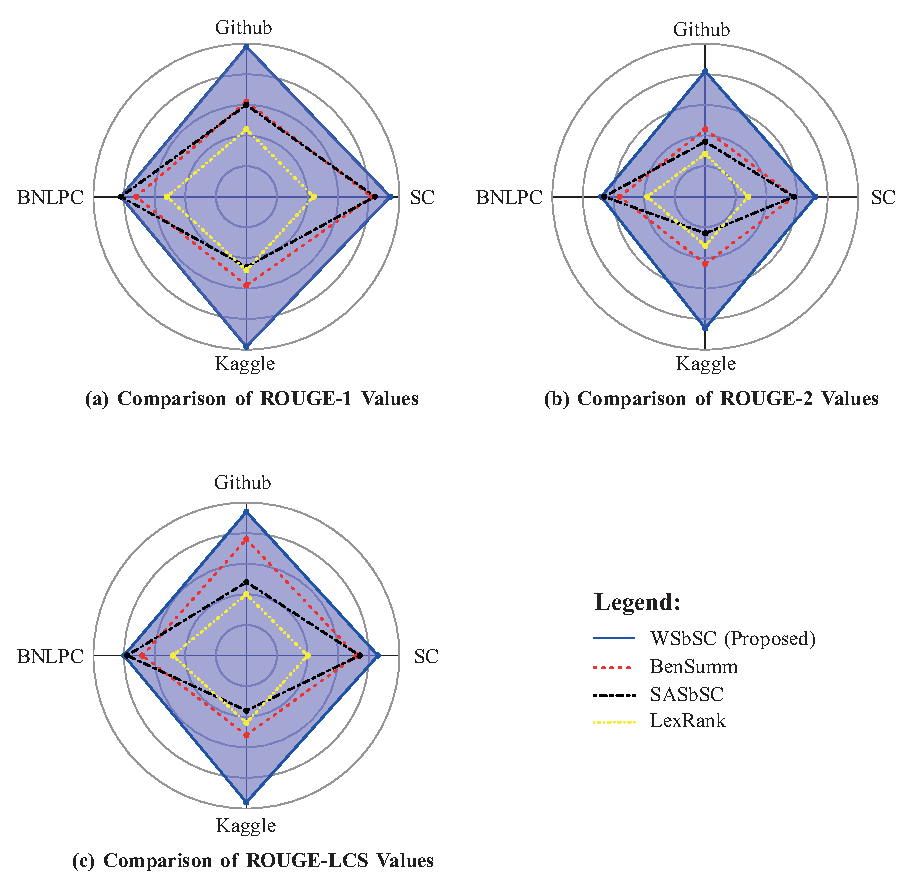
\includegraphics[width=0.8\textwidth]{figs/radar-chart-edited}
	\caption{The Radar chart of the models of being compared on four datasets at once}
	\label{fig:radarchart}
\end{figure}
These results are further visualized into three radar charts in Figure \ref{fig:radarchart} to compare the performance of the models on different Rouge metrics. As stated in the charts, the proposed method performed consistently and uniformly across all the datasets regardless of the quality of the dataset. But other models, such as BenSumm performs well in three datasets (SC, GitHub, BNLPC) but fails in the Kaggle dataset. Similarly, SASbSC performs well in SC and BNLPC datasets but its performance decreases sharply in Kaggle and GitHub datasets. LexRank although performs consistently across all datasets but is far lower on average. According to the result analysis in Table \ref{tab:result_comparison-1} and Figure \ref{fig:radarchart}, WSbSC is the most accurate and reliable Bengali extractive text summarization model.

\subsection{Implementation Into Other Languages}\label{subsec:implementation-into-other-languages}
The proposed model is language-independent thus, it can be extended into other languages too. For this, only a language-specific tokenizer, a stop-word list and a word embedding dataset is required. We implemented this model on three non-bengali datasets to show the language independent nature of the model. To evaluate the quality of the sentence extraction, we tried to find evaluation datasets for summarization on other low resource languages. But could only find relevant datasets in three other languages i.e. Hindi, Marathi and Turkish. We adopted the proposed model into these three low resource languages to check how well it performs.\\

\begin{table}[]
	\centering
	\begin{tabular}{lccc}\hline
		Language              	& Rouge-1   & Rouge-2   & Rouge-LCS \\\hline
		Bengali (Self-curated)	& 0.47      & 0.36      & 0.43      \\
		Bengali (Kaggle)   		& 0.49      & 0.43      & 0.48      \\
		Bengali (BNLPC)   		& 0.41      & 0.34      & 0.40      \\
		Bengali (Github)   		& 0.49      & 0.41      & 0.47      \\
		Bengali (Average)       & 0.47      & 0.38      & 0.44      \\\hline
		Hindi                   & 0.40      & 0.26      & 0.36      \\\hline
		Marathi                 & 0.50	    & 0.42      & 0.50      \\\hline
		Turkish                 & 0.48      & 0.39      & 0.47      \\\hline
	\end{tabular}
	\caption{Comparison of Result of proposed summarization method in other low-resource languages}
	\label{tab:other_language}
\end{table}

The Table \ref{tab:other_language} shows the result of the proposed WSbSC method for extractive summarization in other low resource languages. In this table, we can see that the results on Marathi and Turkish are slightly better than the result on Bengali. Although it performs slightly lower on Hindi, the score is still similar to Bengali. To evaluate the models performance on Hindi, we used a Kaggle dataset\footnote{\textit{https://www.kaggle.com/datasets/disisbig/hindi-text-short-and-large-summarization-corpus/}} produced by Gaurav Arora. For the Marathi, we used another Kaggle dataset\footnote{\textit{https://www.kaggle.com/datasets/ketki19/marathi}} produced by Ketki Nirantar. For the Turkish language, we used a GitHub dataset\footnote{\textit{https://github.com/xtinge/turkish-extractive-summarization-dataset/blob/main/dataset/XTINGE-SUM\_TR\_EXT/xtinge-sum\_tr\_ext.json}} produced by the XTINGE \cite{Demir-2024-xtinge_turkish_extractive} team for evaluation. 

\section{Discussion}\label{sec:discussion}
The results presented at Table \ref{tab:result_comparison-1}, \ref{tab:other_language} and Figure \ref{fig:radarchart} highlights the effectiveness of proposed WSbSC model for extractive text summarization in Bengali, as well as its adaptability to other low-resource languages. This section analyses the comparative results, the strengths and limitations of the proposed method, and potential areas for further research.\\

As evidenced by the results shown in Table~\ref{tab:result_comparison-1} and Figure~\ref{fig:radarchart}, the WSbSC model consistently outperforms other graph-based extractive text summarization models, namely BenSumm \cite{das-2022-tfidf}, LexRank \cite{Erkan-lexRank-2004}, and SASbSC \cite{roychowdhury-etal-2022-spectral-base}, across four datasets. The proposed model shows better performance compared to other three methods on Rouge-1, Rouge-2, Rouge-LCS metrics. This performance improvement can largely be attributed to the novel approach of calculating sentence similarity. While calculating sentence similarity, taking the geometric mean of individual similarity between word pairs overcomes the lack of local word correspondence faced by the averaging vector method \cite{roychowdhury-etal-2022-spectral-base}. The Gaussian kernel-based word similarity provides a precise semantic relationships between sentences which further contribute in the performance improvement. Another reason for performance improvement is the usage of spectral clustering which is very effective in capturing irregular cluster shapes.\\

WSbSC includes a novel strategy for calculating sentence similarity despite the existence of other popular methods for comparing two sets of vectors. Our proposed strategy is more suited for similarity calculation in the context of language than other strategies such as Earth Movers Distance (EMD) \cite{Rubner-19998-emd}, Hausdorff Distance \cite{hausdorff-1914-hausdorff-distance}, Procrustes Analysis \cite{Gower-1975-procrustes-distance}. EMD \cite{Rubner-19998-emd} and Procrustes Analysis \cite{Gower-1975-procrustes-distance} are two very computationally expensive method who also involve scaling or rotating vectors; irrelevant for word vectors due to not holding any semantic meaning. Another method, Hausdorff distance \cite{hausdorff-1914-hausdorff-distance} calculates the highest possible distance between vectors from two set. Although similarly expensive as WSbSC, it is easily influenced by outlier words due to only considering the worst case scenario.\\

On the other hand, the proposed method focuses on local vector similarity between two sets which is more important for words. The Gaussian similarity function captures the proximity of points smoothly, providing a continuous value for similarity between two words in a normalized way. Gaussian similarity is also robust against small outliers due to being a soft similarity measure. Taking geometric mean also helps smooth over similarity values for outlier words.\\

One of the key strengths of this proposed method is the reduction of redundancy, a common challenge in extractive summarization methods, by grouping semantically similar sentences together. The use of spectral clustering for the grouping task improves the performance by not assuming a specific cluster shape. Another key strength of WSbSC is the improved sentence similarity calculation technique over word averaging method \cite{roychowdhury-etal-2022-spectral-base}, which dilutes the semantic meaning of a sentence. Another key strength is the scalability of the method across languages by requiring very few language-specific resources. This scalability is demonstrated in the experiments with Hindi, Marathi, and Turkish languages (Table \ref{tab:other_language}).\\

Despite its advantages, the WSbSC model does face some challenges. The model heavily relies on pre-trained word embeddings, which may not always capture the full details of certain domains or newly coined terms. The FastText \cite{grave-etal-2018-fasttext} dataset used here is heavily reliant on wikipedia for training which could introduce some small unforeseen biases. Where the word embeddings do not have some words of a given document, the model’s performance could degrade as it leaves those words out of the calculation process. The model also does not take into account the order in which words appear in a sentence or when they form special noun or verb groups. So it can be a little naive in some highly specialized fields.\\

The proposed WSbSC model represents a significant advancement in Bengali extractive text summarization due to its ability to accurately capture semantic similarity, reduce redundancy, maximize coverage and generalize across languages. While there are still challenges to be addressed, the results of this study demonstrate the robustness and adaptability of the WSbSC model, offering a promising direction for future research in multilingual extractive summarization.

\section{Conclusion}\label{sec:conclusion}
In this study, we proposed a Word Similarity-based Spectral Clustering (WSbSC) method for Bengali extractive text summarization which can also be used in other low resource languages. the proposed method used geometric mean of Gaussian similarities between individual word pairs to identify deeper semantic relationship within two sentences. This method for calculating sentence similarity helps WSbSC to significantly outperform other recent graph based extractive text summarization methods on four varying datasets with different sizes and sources. This improvement in performance is also helped by the use of spectral clustering which helps to improve coherence and relevance of the generated summaries by minimizing redundancy and maximizing topic coverage. High performance across three ROUGE metrics on four datasets prove the versatility and robustness of the proposed method. WSbSC can also be extended into other languages as shown through our experimentations on Hindi, Marathi and Turkish languages proving the generalizability of the method. This method addresses the need for an effective summarization technique in Bengali language as Bengali remains under-represented in NLP research despite it being the 7th largest language in the world.\\

Through results of extensive experimentations, we showed the strengths of the proposed WSbSC method as it outperforms several baseline techniques using a better approach to grouping sentences into key topics. Despite these promising results, there are areas with limitation that requires further improvement. WSbSC may face limitations on highly specialized or domain-specific texts, where deeper linguistic features beyond word similarity could be considered. The lack of consideration for word order in a sentence is also a key limitation which could be explored in the future. Future works could also explore hybrid models that integrate modern post-processing techniques to improve the flow of the output.\\

In conclusion, this work contributes to the growing body of computational linguistics research focused on low-resource languages like Bengali. The WSbSC method offers a novel approach for extractive summarization by using a new algorithm for calculating similarity between two sentences and sets the stage for further advancements in both Bengali text processing and multilingual summarization techniques.

















































\begin{comment}

	\section{Template Overview}
	As noted in the introduction, the ``\verb|acmart|'' document class can
	be used to prepare many different kinds of documentation --- a
	double-anonymous initial submission of a full-length technical paper, a
	two-page SIGGRAPH Emerging Technologies abstract, a ``camera-ready''
	journal article, a SIGCHI Extended Abstract, and more --- all by
	selecting the appropriate {\itshape template style} and {\itshape
	  template parameters}.
	
	This document will explain the major features of the document
	class. For further information, the {\itshape \LaTeX\ User's Guide} is
	available from
	\url{https://www.acm.org/publications/proceedings-template}.
	
	\subsection{Template Styles}
	
	The primary parameter given to the ``\verb|acmart|'' document class is
	the {\itshape template style} which corresponds to the kind of publication
	or SIG publishing the work. This parameter is enclosed in square
	brackets and is a part of the {\verb|documentclass|} command:
	\begin{verbatim}
	  \documentclass[STYLE]{acmart}
	\end{verbatim}
	
	Journals use one of three template styles. All but three ACM journals
	use the {\verb|acmsmall|} template style:
	\begin{itemize}
	\item {\texttt{acmsmall}}: The default journal template style.
	\item {\texttt{acmlarge}}: Used by JOCCH and TAP.
	\item {\texttt{acmtog}}: Used by TOG.
	\end{itemize}
	
	The majority of conference proceedings documentation will use the {\verb|acmconf|} template style.
	\begin{itemize}
	\item {\texttt{sigconf}}: The default proceedings template style.
	\item{\texttt{sigchi}}: Used for SIGCHI conference articles.
	\item{\texttt{sigplan}}: Used for SIGPLAN conference articles.
	\end{itemize}
	
	\subsection{Template Parameters}
	
	In addition to specifying the {\itshape template style} to be used in
	formatting your work, there are a number of {\itshape template parameters}
	which modify some part of the applied template style. A complete list
	of these parameters can be found in the {\itshape \LaTeX\ User's Guide.}
	
	Frequently-used parameters, or combinations of parameters, include:
	\begin{itemize}
	\item {\texttt{anonymous,review}}: Suitable for a ``double-anonymous''
	  conference submission. Anonymizes the work and includes line
	  numbers. Use with the \texttt{\acmSubmissionID} command to print the
	  submission's unique ID on each page of the work.
	\item{\texttt{authorversion}}: Produces a version of the work suitable
	  for posting by the author.
	\item{\texttt{screen}}: Produces colored hyperlinks.
	\end{itemize}
	
	This document uses the following string as the first command in the
	source file:
	\begin{verbatim}
	\documentclass[acmlarge]{acmart}
	\end{verbatim}
	
	\section{Modifications}
	
	Modifying the template --- including but not limited to: adjusting
	margins, typeface sizes, line spacing, paragraph and list definitions,
	and the use of the \verb|\vspace| command to manually adjust the
	vertical spacing between elements of your work --- is not allowed.
	
	{\bfseries Your document will be returned to you for revision if
	  modifications are discovered.}
	
	\section{Typefaces}
	
	The ``\verb|acmart|'' document class requires the use of the
	``Libertine'' typeface family. Your \TeX\ installation should include
	this set of packages. Please do not substitute other typefaces. The
	``\verb|lmodern|'' and ``\verb|ltimes|'' packages should not be used,
	as they will override the built-in typeface families.
	
	\section{Title Information}
	
	The title of your work should use capital letters appropriately -
	\url{https://capitalizemytitle.com/} has useful rules for
	capitalization. Use the {\verb|title|} command to define the title of
	your work. If your work has a subtitle, define it with the
	{\verb|subtitle|} command.  Do not insert line breaks in your title.
	
	If your title is lengthy, you must define a short version to be used
	in the page headers, to prevent overlapping text. The \verb|title|
	command has a ``short title'' parameter:
	\begin{verbatim}
	  \title[short title]{full title}
	\end{verbatim}
	
	\section{Authors and Affiliations}
	
	Each author must be defined separately for accurate metadata
	identification.  As an exception, multiple authors may share one
	affiliation. Authors' names should not be abbreviated; use full first
	names wherever possible. Include authors' e-mail addresses whenever
	possible.
	
	Grouping authors' names or e-mail addresses, or providing an ``e-mail
	alias,'' as shown below, is not acceptable:
	\begin{verbatim}
	  \author{Brooke Aster, David Mehldau}
	  \email{dave,judy,steve@university.edu}
	  \email{firstname.lastname@phillips.org}
	\end{verbatim}
	
	The \verb|authornote| and \verb|authornotemark| commands allow a note
	to apply to multiple authors --- for example, if the first two authors
	of an article contributed equally to the work.
	
	If your author list is lengthy, you must define a shortened version of
	the list of authors to be used in the page headers, to prevent
	overlapping text. The following command should be placed just after
	the last \verb|\author{}| definition:
	\begin{verbatim}
	  \renewcommand{\shortauthors}{McCartney, et al.}
	\end{verbatim}
	Omitting this command will force the use of a concatenated list of all
	of the authors' names, which may result in overlapping text in the
	page headers.
	
	The article template's documentation, available at
	\url{https://www.acm.org/publications/proceedings-template}, has a
	complete explanation of these commands and tips for their effective
	use.
	
	Note that authors' addresses are mandatory for journal articles.
	
	\section{Rights Information}
	
	Authors of any work published by ACM will need to complete a rights
	form. Depending on the kind of work, and the rights management choice
	made by the author, this may be copyright transfer, permission,
	license, or an OA (open access) agreement.
	
	Regardless of the rights management choice, the author will receive a
	copy of the completed rights form once it has been submitted. This
	form contains \LaTeX\ commands that must be copied into the source
	document. When the document source is compiled, these commands and
	their parameters add formatted text to several areas of the final
	document:
	\begin{itemize}
	\item the ``ACM Reference Format'' text on the first page.
	\item the ``rights management'' text on the first page.
	\item the conference information in the page header(s).
	\end{itemize}
	
	Rights information is unique to the work; if you are preparing several
	works for an event, make sure to use the correct set of commands with
	each of the works.
	
	The ACM Reference Format text is required for all articles over one
	page in length, and is optional for one-page articles (abstracts).
	
	\section{CCS Concepts and User-Defined Keywords}
	
	Two elements of the ``acmart'' document class provide powerful
	taxonomic tools for you to help readers find your work in an online
	search.
	
	The ACM Computing Classification System ---
	\url{https://www.acm.org/publications/class-2012} --- is a set of
	classifiers and concepts that describe the computing
	discipline. Authors can select entries from this classification
	system, via \url{https://dl.acm.org/ccs/ccs.cfm}, and generate the
	commands to be included in the \LaTeX\ source.
	
	User-defined keywords are a comma-separated list of words and phrases
	of the authors' choosing, providing a more flexible way of describing
	the research being presented.
	
	CCS concepts and user-defined keywords are required for for all
	articles over two pages in length, and are optional for one- and
	two-page articles (or abstracts).
	
	\section{Sectioning Commands}
	
	Your work should use standard \LaTeX\ sectioning commands:
	\verb|section|, \verb|subsection|, \verb|subsubsection|, and
	\verb|paragraph|. They should be numbered; do not remove the numbering
	from the commands.
	
	Simulating a sectioning command by setting the first word or words of
	a paragraph in boldface or italicized text is {\bfseries not allowed.}
	
	\section{Tables}
	
	The ``\verb|acmart|'' document class includes the ``\verb|booktabs|''
	package --- \url{https://ctan.org/pkg/booktabs} --- for preparing
	high-quality tables.
	
	Table captions are placed {\itshape above} the table.
	
	Because tables cannot be split across pages, the best placement for
	them is typically the top of the page nearest their initial cite.  To
	ensure this proper ``floating'' placement of tables, use the
	environment \textbf{table} to enclose the table's contents and the
	table caption.  The contents of the table itself must go in the
	\textbf{tabular} environment, to be aligned properly in rows and
	columns, with the desired horizontal and vertical rules.  Again,
	detailed instructions on \textbf{tabular} material are found in the
	\textit{\LaTeX\ User's Guide}.
	
	Immediately following this sentence is the point at which
	Table~\ref{tab:freq} is included in the input file; compare the
	placement of the table here with the table in the printed output of
	this document.
	
	\begin{table}
	  \caption{Frequency of Special Characters}
	  \label{tab:freq}
	  \begin{tabular}{ccl}
	    \toprule
	    Non-English or Math&Frequency&Comments\\
	    \midrule
	    \O & 1 in 1,000& For Swedish names\\
	    $\pi$ & 1 in 5& Common in math\\
	    \$ & 4 in 5 & Used in business\\
	    $\Psi^2_1$ & 1 in 40,000& Unexplained usage\\
	  \bottomrule
	\end{tabular}
	\end{table}
	
	To set a wider table, which takes up the whole width of the page's
	live area, use the environment \textbf{table*} to enclose the table's
	contents and the table caption.  As with a single-column table, this
	wide table will ``float'' to a location deemed more
	desirable. Immediately following this sentence is the point at which
	Table~\ref{tab:commands} is included in the input file; again, it is
	instructive to compare the placement of the table here with the table
	in the printed output of this document.
	
	\begin{table*}
	  \caption{Some Typical Commands}
	  \label{tab:commands}
	  \begin{tabular}{ccl}
	    \toprule
	    Command &A Number & Comments\\
	    \midrule
	    \texttt{{\char'134}author} & 100& Author \\
	    \texttt{{\char'134}table}& 300 & For tables\\
	    \texttt{{\char'134}table*}& 400& For wider tables\\
	    \bottomrule
	  \end{tabular}
	\end{table*}
	
	Always use midrule to separate table header rows from data rows, and
	use it only for this purpose. This enables assistive technologies to
	recognise table headers and support their users in navigating tables
	more easily.
	
	\section{Math Equations}
	You may want to display math equations in three distinct styles:
	inline, numbered or non-numbered display.  Each of the three are
	discussed in the next sections.
	
	\subsection{Inline (In-text) Equations}
	A formula that appears in the running text is called an inline or
	in-text formula.  It is produced by the \textbf{math} environment,
	which can be invoked with the usual
	\texttt{{\char'134}begin\,\ldots{\char'134}end} construction or with
	the short form \texttt{\$\,\ldots\$}. You can use any of the symbols
	and structures, from $\alpha$ to $\omega$, available in
	\LaTeX~\cite{Lamport:LaTeX}; this section will simply show a few
	examples of in-text equations in context. Notice how this equation:
	\begin{math}
	  \lim_{n\rightarrow \infty}x=0
	\end{math},
	set here in in-line math style, looks slightly different when
	set in display style.  (See next section).
	
	\subsection{Display Equations}
	A numbered display equation---one set off by vertical space from the
	text and centered horizontally---is produced by the \textbf{equation}
	environment. An unnumbered display equation is produced by the
	\textbf{displaymath} environment.
	
	Again, in either environment, you can use any of the symbols and
	structures available in \LaTeX\@; this section will just give a couple
	of examples of display equations in context.  First, consider the
	equation, shown as an inline equation above:
	\begin{equation}
	  \lim_{n\rightarrow \infty}x=0
	\end{equation}
	Notice how it is formatted somewhat differently in
	the \textbf{displaymath}
	environment.  Now, we'll enter an unnumbered equation:
	\begin{displaymath}
	  \sum_{i=0}^{\infty} x + 1
	\end{displaymath}
	and follow it with another numbered equation:
	\begin{equation}
	  \sum_{i=0}^{\infty}x_i=\int_{0}^{\pi+2} f
	\end{equation}
	just to demonstrate \LaTeX's able handling of numbering.
	
	\section{Figures}
	
	The ``\verb|figure|'' environment should be used for figures. One or
	more images can be placed within a figure. If your figure contains
	third-party material, you must clearly identify it as such, as shown
	in the example below.
	\begin{figure}[h]
	  \centering
	  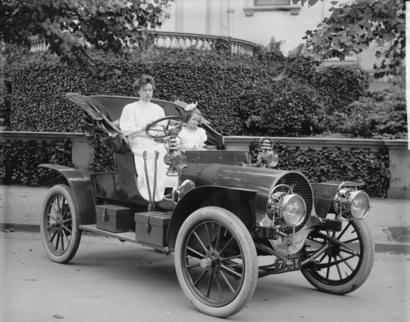
\includegraphics[width=\linewidth]{sample-franklin}
	  \caption{1907 Franklin Model D roadster. Photograph by Harris \&
	    Ewing, Inc. [Public domain], via Wikimedia
	    Commons. (\url{https://goo.gl/VLCRBB}).}
	  \Description{A woman and a girl in white dresses sit in an open car.}
	\end{figure}
	
	Your figures should contain a caption which describes the figure to
	the reader.
	
	Figure captions are placed {\itshape below} the figure.
	
	Every figure should also have a figure description unless it is purely
	decorative. These descriptions convey what’s in the image to someone
	who cannot see it. They are also used by search engine crawlers for
	indexing images, and when images cannot be loaded.
	
	A figure description must be unformatted plain text less than 2000
	characters long (including spaces).  {\bfseries Figure descriptions
	  should not repeat the figure caption – their purpose is to capture
	  important information that is not already provided in the caption or
	  the main text of the paper.} For figures that convey important and
	complex new information, a short text description may not be
	adequate. More complex alternative descriptions can be placed in an
	appendix and referenced in a short figure description. For example,
	provide a data table capturing the information in a bar chart, or a
	structured list representing a graph.  For additional information
	regarding how best to write figure descriptions and why doing this is
	so important, please see
	\url{https://www.acm.org/publications/taps/describing-figures/}.
	
	\subsection{The ``Teaser Figure''}
	
	A ``teaser figure'' is an image, or set of images in one figure, that
	are placed after all author and affiliation information, and before
	the body of the article, spanning the page. If you wish to have such a
	figure in your article, place the command immediately before the
	\verb|\maketitle| command:
	\begin{verbatim}
	  \begin{teaserfigure}
	    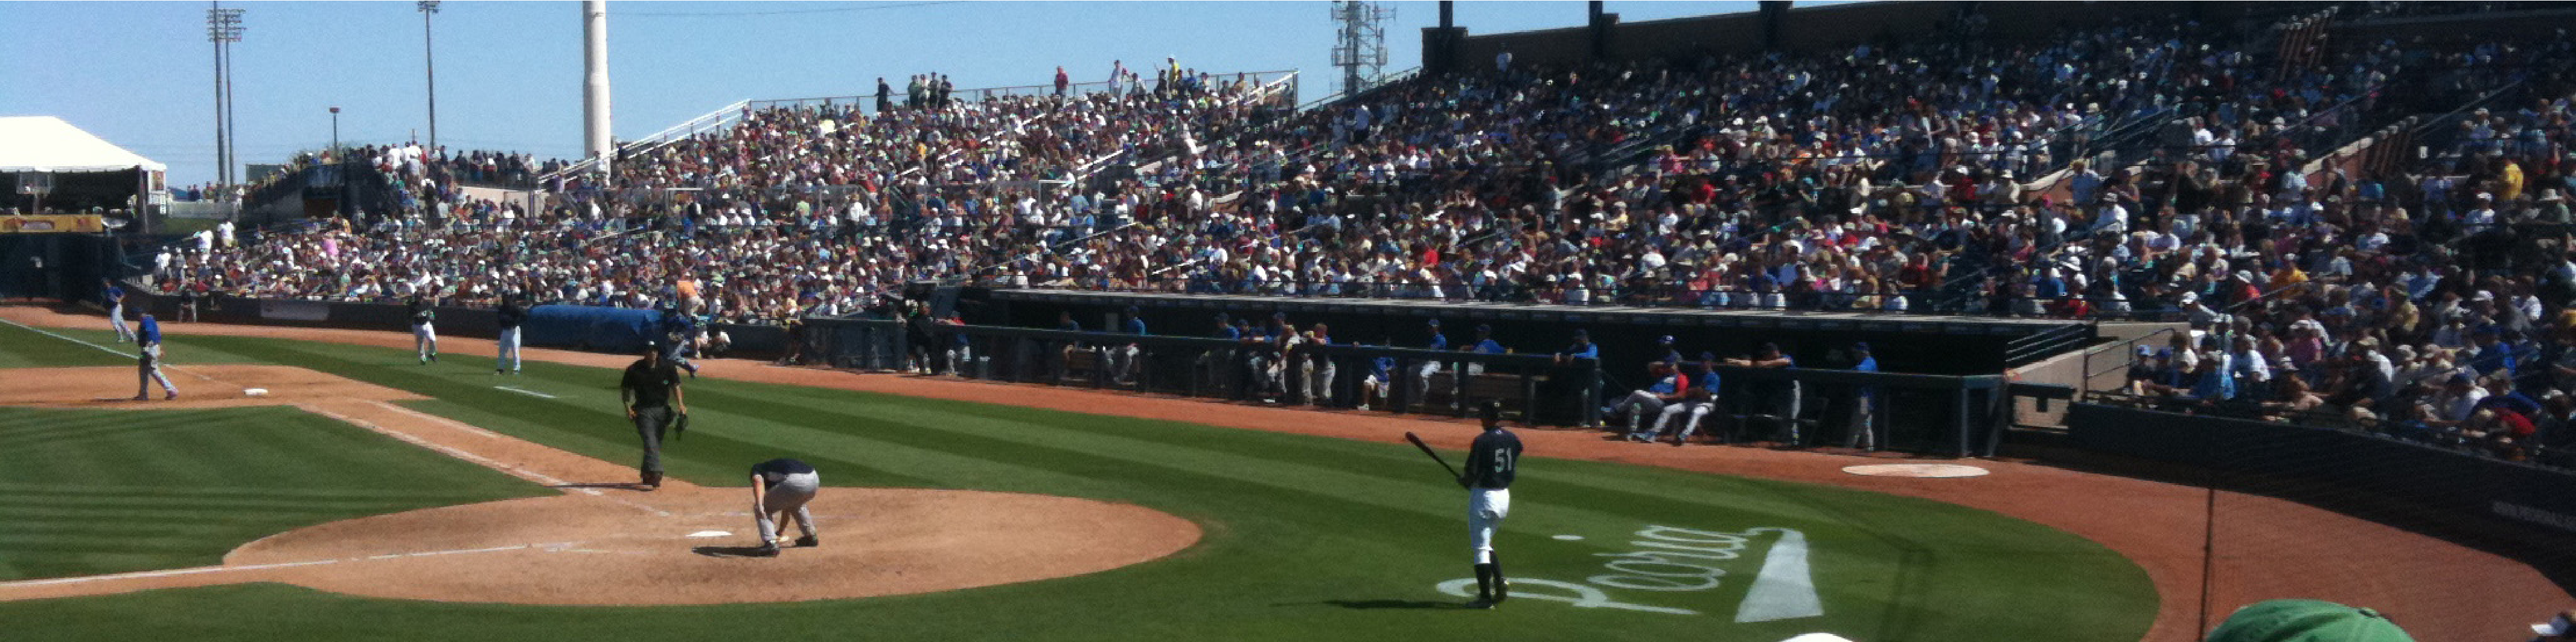
\includegraphics[width=\textwidth]{sampleteaser}
	    \caption{figure caption}
	    \Description{figure description}
	  \end{teaserfigure}
	\end{verbatim}
	
	\section{Citations and Bibliographies}
	
	The use of \BibTeX\ for the preparation and formatting of one's
	references is strongly recommended. Authors' names should be complete
	--- use full first names (``Donald E. Knuth'') not initials
	(``D. E. Knuth'') --- and the salient identifying features of a
	reference should be included: title, year, volume, number, pages,
	article DOI, etc.
	
	The bibliography is included in your source document with these two
	commands, placed just before the \verb|\end{document}| command:
	\begin{verbatim}
	  \bibliographystyle{ACM-Reference-Format}
	  \bibliography{bibfile}
	\end{verbatim}
	where ``\verb|bibfile|'' is the name, without the ``\verb|.bib|''
	suffix, of the \BibTeX\ file.
	
	Citations and references are numbered by default. A small number of
	ACM publications have citations and references formatted in the
	``author year'' style; for these exceptions, please include this
	command in the {\bfseries preamble} (before the command
	``\verb|\begin{document}|'') of your \LaTeX\ source:
	\begin{verbatim}
	  \citestyle{acmauthoryear}
	\end{verbatim}
	
	
	  Some examples.  A paginated journal article \cite{Abril07}, an
	  enumerated journal article \cite{Cohen07}, a reference to an entire
	  issue \cite{JCohen96}, a monograph (whole book) \cite{Kosiur01}, a
	  monograph/whole book in a series (see 2a in spec. document)
	  \cite{Harel79}, a divisible-book such as an anthology or compilation
	  \cite{Editor00} followed by the same example, however we only output
	  the series if the volume number is given \cite{Editor00a} (so
	  Editor00a's series should NOT be present since it has no vol. no.),
	  a chapter in a divisible book \cite{Spector90}, a chapter in a
	  divisible book in a series \cite{Douglass98}, a multi-volume work as
	  book \cite{Knuth97}, a couple of articles in a proceedings (of a
	  conference, symposium, workshop for example) (paginated proceedings
	  article) \cite{Andler79, Hagerup1993}, a proceedings article with
	  all possible elements \cite{Smith10}, an example of an enumerated
	  proceedings article \cite{VanGundy07}, an informally published work
	  \cite{Harel78}, a couple of preprints \cite{Bornmann2019,
	    AnzarootPBM14}, a doctoral dissertation \cite{Clarkson85}, a
	  master's thesis: \cite{anisi03}, an online document / world wide web
	  resource \cite{Thornburg01, Ablamowicz07, Poker06}, a video game
	  (Case 1) \cite{Obama08} and (Case 2) \cite{Novak03} and \cite{Lee05}
	  and (Case 3) a patent \cite{JoeScientist001}, work accepted for
	  publication \cite{rous08}, 'YYYYb'-test for prolific author
	  \cite{SaeediMEJ10} and \cite{SaeediJETC10}. Other cites might
	  contain 'duplicate' DOI and URLs (some SIAM articles)
	  \cite{Kirschmer:2010:AEI:1958016.1958018}. Boris / Barbara Beeton:
	  multi-volume works as books \cite{MR781536} and \cite{MR781537}. A
	  couple of citations with DOIs:
	  \cite{2004:ITE:1009386.1010128,Kirschmer:2010:AEI:1958016.1958018}. Online
	  citations: \cite{TUGInstmem, Thornburg01, CTANacmart}.
	  Artifacts: \cite{R} and \cite{UMassCitations}.
	
	\section{Acknowledgments}
	
	Identification of funding sources and other support, and thanks to
	individuals and groups that assisted in the research and the
	preparation of the work should be included in an acknowledgment
	section, which is placed just before the reference section in your
	document.
	
	This section has a special environment:
	\begin{verbatim}
	  \begin{acks}
	  ...
	  \end{acks}
	\end{verbatim}
	so that the information contained therein can be more easily collected
	during the article metadata extraction phase, and to ensure
	consistency in the spelling of the section heading.
	
	Authors should not prepare this section as a numbered or unnumbered {\verb|\section|}; please use the ``{\verb|acks|}'' environment.
	
	\section{Appendices}
	
	If your work needs an appendix, add it before the
	``\verb|\end{document}|'' command at the conclusion of your source
	document.
	
	Start the appendix with the ``\verb|appendix|'' command:
	\begin{verbatim}
	  \appendix
	\end{verbatim}
	and note that in the appendix, sections are lettered, not
	numbered. This document has two appendices, demonstrating the section
	and subsection identification method.
	
	\section{Multi-language papers}
	
	Papers may be written in languages other than English or include
	titles, subtitles, keywords and abstracts in different languages (as a
	rule, a paper in a language other than English should include an
	English title and an English abstract).  Use \verb|language=...| for
	every language used in the paper.  The last language indicated is the
	main language of the paper.  For example, a French paper with
	additional titles and abstracts in English and German may start with
	the following command
	\begin{verbatim}
	\documentclass[sigconf, language=english, language=german,
	               language=french]{acmart}
	\end{verbatim}
	
	The title, subtitle, keywords and abstract will be typeset in the main
	language of the paper.  The commands \verb|\translatedXXX|, \verb|XXX|
	begin title, subtitle and keywords, can be used to set these elements
	in the other languages.  The environment \verb|translatedabstract| is
	used to set the translation of the abstract.  These commands and
	environment have a mandatory first argument: the language of the
	second argument.  See \verb|sample-sigconf-i13n.tex| file for examples
	of their usage.
	
	\section{SIGCHI Extended Abstracts}
	
	The ``\verb|sigchi-a|'' template style (available only in \LaTeX\ and
	not in Word) produces a landscape-orientation formatted article, with
	a wide left margin. Three environments are available for use with the
	``\verb|sigchi-a|'' template style, and produce formatted output in
	the margin:
	\begin{description}
	\item[\texttt{sidebar}:]  Place formatted text in the margin.
	\item[\texttt{marginfigure}:] Place a figure in the margin.
	\item[\texttt{margintable}:] Place a table in the margin.
	\end{description}
	
	%%
	%% The acknowledgments section is defined using the "acks" environment
	%% (and NOT an unnumbered section). This ensures the proper
	%% identification of the section in the article metadata, and the
	%% consistent spelling of the heading.
	\begin{acks}
	To Robert, for the bagels and explaining CMYK and color spaces.
	\end{acks}
	
	%%
	%% The next two lines define the bibliography style to be used, and
	%% the bibliography file.
	
\end{comment}
\bibliographystyle{ACM-Reference-Format}
\bibliography{main}


%%
%% If your work has an appendix, this is the place to put it.
\appendix
\begin{comment}
	
\section{Research Methods}

\subsection{Part One}

Lorem ipsum dolor sit amet, consectetur adipiscing elit. Morbi
malesuada, quam in pulvinar varius, metus nunc fermentum urna, id
sollicitudin purus odio sit amet enim. Aliquam ullamcorper eu ipsum
vel mollis. Curabitur quis dictum nisl. Phasellus vel semper risus, et
lacinia dolor. Integer ultricies commodo sem nec semper.

\subsection{Part Two}

Etiam commodo feugiat nisl pulvinar pellentesque. Etiam auctor sodales
ligula, non varius nibh pulvinar semper. Suspendisse nec lectus non
ipsum convallis congue hendrerit vitae sapien. Donec at laoreet
eros. Vivamus non purus placerat, scelerisque diam eu, cursus
ante. Etiam aliquam tortor auctor efficitur mattis.

\section{Online Resources}

Nam id fermentum dui. Suspendisse sagittis tortor a nulla mollis, in
pulvinar ex pretium. Sed interdum orci quis metus euismod, et sagittis
enim maximus. Vestibulum gravida massa ut felis suscipit
congue. Quisque mattis elit a risus ultrices commodo venenatis eget
dui. Etiam sagittis eleifend elementum.

Nam interdum magna at lectus dignissim, ac dignissim lorem
rhoncus. Maecenas eu arcu ac neque placerat aliquam. Nunc pulvinar
massa et mattis lacinia.

\end{comment}

\end{document}
\endinput
%%
%% End of file `sample-acmlarge.tex'.
